\section{Sistema de inyección electrónica}
\subsection{Evolución de los sistemas de alimentación de combustible}


La evolución de los sistemas de alimentación de combustible en los vehículos ha pasado desde el carburador mecánico hasta sistemas electrónicos de inyección monopunto, multipunto e inyección directa, cada uno asociado a cambios normativos sobre emisiones y avances en electrónica del motor\citep{web1,web10,web14}.

\begin{itemize}
    \item \textbf{Finales del siglo XIX -- 1900}:  
    Los primeros motores de gasolina utilizan mezcladores mecánicos rudimentarios; el carburador se consolida como dispositivo estándar para crear la mezcla aire–combustible\citep{web10, web14}.

    \item \textbf{1912 -- 1930s}:  
    Primeros ensayos de bombas de inyección de gasolina en motores de aviación; en 1937 se aplica en serie la inyección de combustible en motores de avión, sentando las bases para los sistemas de inyección modernos\citep{web14}.

    \item \textbf{1945 -- 1950s}:  
    Primera aplicación en serie de inyección de gasolina en vehículos de carretera; se mantienen sistemas principalmente mecánicos o electromecánicos, usados en modelos deportivos o de alta gama\citep{web14}.

    \item \textbf{1967}:  
    Bosch introduce el sistema D‑Jetronic, el primer sistema de inyección electrónica de gasolina de producción masiva, sustituyendo parcialmente al carburador en Europa\citep{web1}.

    \item \textbf{1970s}:  
    La crisis del petróleo y las normas de emisiones obligan a abandonar parcialmente el carburador; se extienden sistemas de inyección electrónica continuos (por ejemplo KE‑Jetronic) y se empiezan a usar en modelos de serie de fabricantes como Mercedes‑Benz y otros\citep{web1,web14}.

    \item \textbf{1980s}:  
    Aparecen sistemas digitales de gestión del motor (por ejemplo Motronic de Bosch), integrando inyección electrónica multipunto y encendido electrónico; marcas como Volkswagen, BMW y Mercedes adoptan estos sistemas en múltiples modelos\citep{web7}.

    \item \textbf{1990}:  
    Se difunden sistemas de inyección electrónica monopunto y multipunto indirecta en vehículos comerciales de bajo costo (por ejemplo Suzuki Samurai 1990 y Suzuki Jimny 2000)\citep{web10}.

    \item \textbf{1990s -- 2000s}:  
    Implantación masiva del carburador en motores de gasolina reemplazado por inyección electrónica multipunto (por ejemplo General Motors, Ford, Honda, etc.); se adopta el catalizador de tres vías, lo que exige un control muy preciso de la mezcla aire–combustible\citep{web1,web7,web10}.

    \item \textbf{2000s -- 2010s}:  
    Desarrollo de sistemas de inyección directa de gasolina (GDI) en modelos de alta eficiencia y potencia (por ejemplo Toyota, Mazda, BMW, VW, GM); se combinan turbocompresores y control electrónico avanzado para reducir consumo y emisiones\citep{web1,web7}.

    \item \textbf{2010 -- actualidad}:  
    La inyección directa se vuelve estándar en muchos motores de gasolina y se introducen sistemas flexibles de inyección múltiple por ciclo, combinados con sistemas híbridos y electrificación parcial de la alimentación (bomba eléctrica de alta presión, inyección piezoeléctrica en diesel)\citep{web1,web7}.
\end{itemize}

\begin{figure}[h]
	\centering
	
	% 1. El caption automático estilo APA 7 (Título conciso arriba)
	\caption{Línea de tiempo de la evolución en los sistemas de alimentación de combustible}
	\label{fig:evolucion_combustible}
	\vspace{0.3cm}
	
	% 2. La imagen ajustada exactamente al límite del margen del texto
	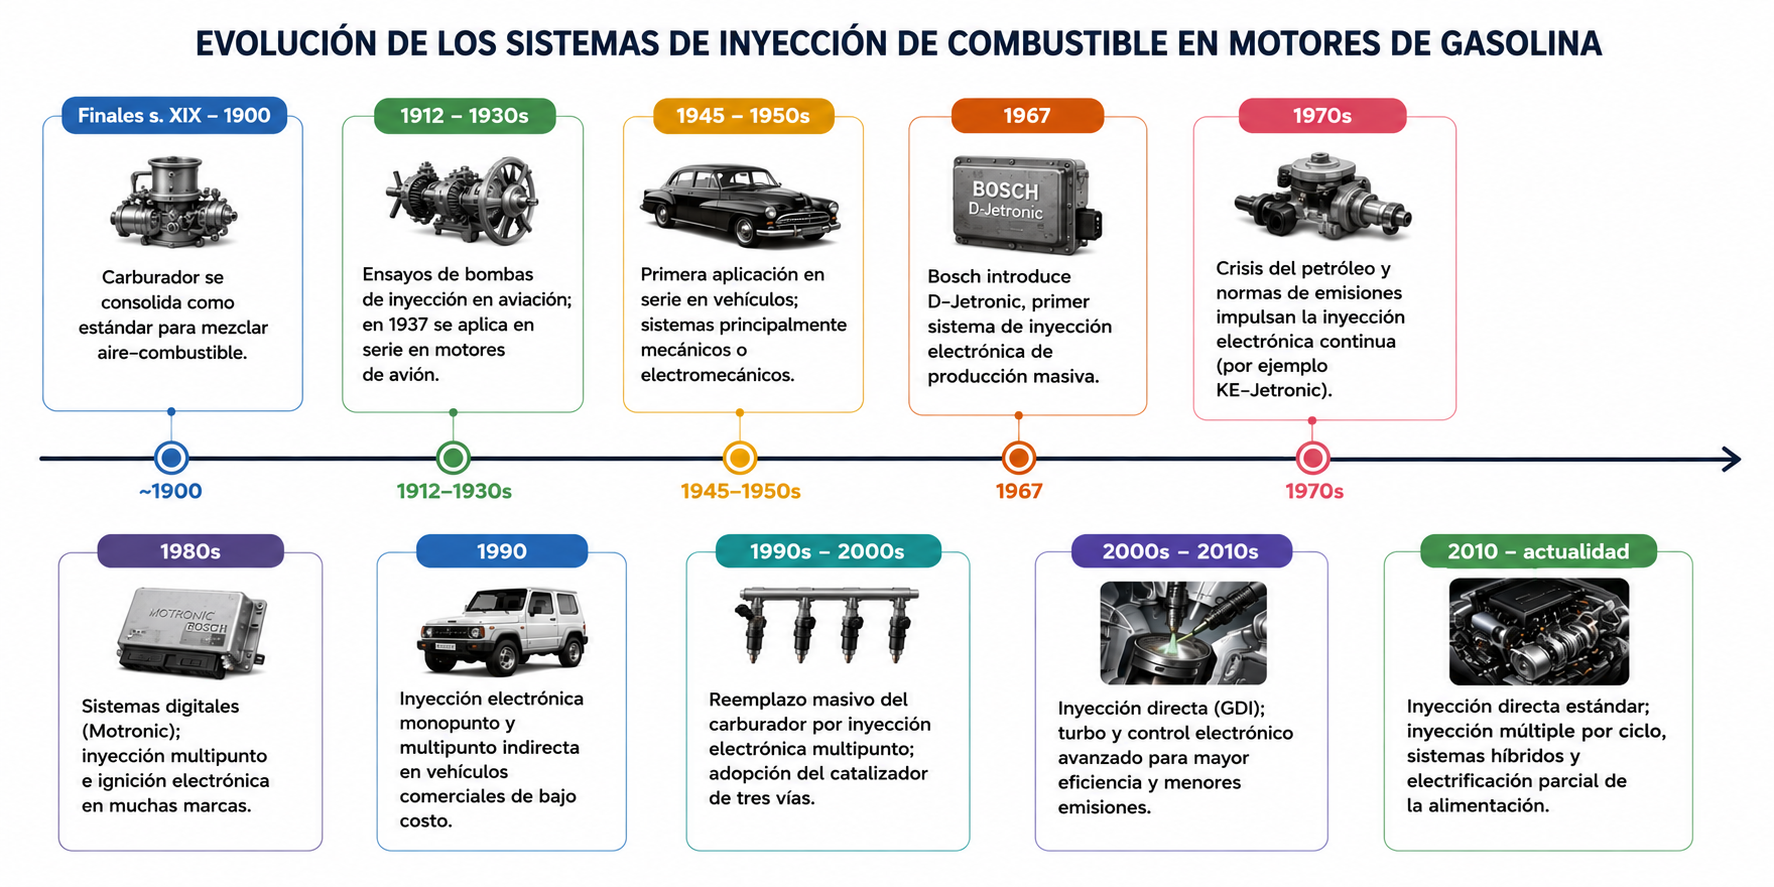
\includegraphics[width=1.0\textwidth]{Images/LINEA.png}
	\vspace{0.2cm}
	
	% 3. La nota de la figura según APA 7 (Con descripción técnica)
	\begin{flushleft}
		\footnotesize \textit{Nota.} Cronología del desarrollo tecnológico en la dosificación de combustible, destacando la transición desde sistemas mecánicos por carburador hasta esquemas de inyección electrónica directa controlados por computadora. Elaboración propia con base en \citep{web1}, \citep{web10} y \citep{web7}.
	\end{flushleft}
\end{figure}

\subsection{Tipos de sistemas de inyección electrónica}% (monopunto, multipunto, directa)

Los sistemas de inyección electrónica pueden clasificarse según la forma en que suministran el combustible hacia el motor. Entre los más utilizados se encuentran la inyección monopunto, multipunto y directa, cada una con diferentes características de funcionamiento, eficiencia y complejidad tecnológica \citep{Bosch_Automotive, web_inyeccion1}.

\subsubsection{Inyección monopunto}

La inyección monopunto, también conocida como \textit{Single Point Injection} (SPI) o \textit{Throttle Body Injection} (TBI), utiliza un único inyector ubicado en el cuerpo de aceleración para suministrar combustible a todos los cilindros del motor. Su funcionamiento es similar al carburador, pero con control electrónico de la dosificación de combustible \citep{Bosch_Automotive}.

Este sistema fue ampliamente utilizado durante la transición entre carburadores y sistemas de inyección electrónica modernos debido a su bajo costo y simplicidad. Sin embargo, presenta menor precisión en la distribución del combustible y menor eficiencia energética en comparación con sistemas más avanzados \citep{web_inyeccion2}.

Entre sus principales ventajas se encuentran:
\begin{itemize}
    \item Menor costo de implementación.
    \item Diseño simple y mantenimiento reducido.
    \item Mejor control de emisiones respecto al carburador.
\end{itemize}

No obstante, sus desventajas incluyen:
\begin{itemize}
    \item Distribución desigual del combustible.
    \item Menor rendimiento y eficiencia.
    \item Mayor consumo comparado con sistemas modernos.
\end{itemize}

\subsubsection{Inyección multipunto}

La inyección multipunto o \textit{Multi Point Injection} (MPI) emplea un inyector independiente para cada cilindro del motor. Los inyectores se encuentran ubicados en el múltiple de admisión, permitiendo una dosificación más precisa de combustible hacia cada cilindro \citep{Bosch_Automotive, web_inyeccion1}.

Este sistema mejora significativamente el rendimiento del motor, el consumo de combustible y las emisiones contaminantes. Dependiendo de la estrategia de control de la ECU, la inyección puede realizarse de forma simultánea, secuencial o semisecuencial \citep{web_inyeccion2}.

Entre sus ventajas destacan:
\begin{itemize}
    \item Mejor atomización y distribución del combustible.
    \item Reducción del consumo y emisiones.
    \item Mayor eficiencia y respuesta del motor.
\end{itemize}

Sin embargo:
\begin{itemize}
    \item Requiere mayor cantidad de sensores y componentes electrónicos.
    \item Presenta mayor complejidad de diagnóstico y mantenimiento.
\end{itemize}

\subsubsection{Diferencia entre monopunto y multipunto}
De acuerdo con Motorpasión, la inyección directa puede considerarse una evolución de la inyección multipunto, debido a que ambos sistemas utilizan un inyector por cilindro, pero difieren principalmente en la ubicación donde se introduce el combustible. En la inyección multipunto, el combustible es suministrado en el colector de admisión antes de ingresar a la cámara de combustión ver Figura \ref{fig:Multi}, mientras que en la inyección directa el combustible es pulverizado directamente dentro del cilindro, permitiendo una combustión más eficiente y un mejor aprovechamiento energético \citep{Motorpasion_Inyeccion}.

\begin{figure}[h]
	\centering
	
	% 1. El caption automático estilo APA 7 (Título conciso arriba)
	\caption{Diferencias estructurales entre los sistemas de inyección monopunto y multipunto}
	\label{fig:Multi}
	\vspace{0.3cm}
	
	% 2. La imagen ajustada proporcionalmente al ancho del texto
	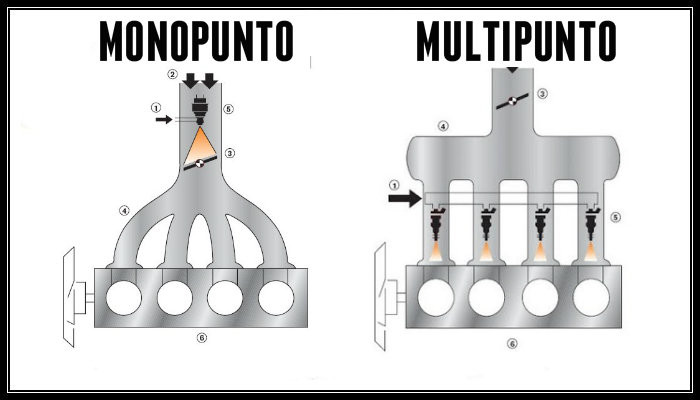
\includegraphics[width=0.6\textwidth]{Images/MULTI.jpg}
	\vspace{0.2cm}
	
	% 3. La nota de la figura según APA 7 (Con descripción técnica)
	\begin{flushleft}
		\footnotesize \textit{Nota.} Comparación esquemática del posicionamiento y cantidad de inyectores en la galería de admisión, contrastando el suministro centralizado (monopunto) frente al flujo independiente por cilindro (multipunto). Tomado de \citep{Motorpasion_Inyeccion}.
	\end{flushleft}
\end{figure}

\subsubsection{Inyección directa}

La inyección directa de gasolina o \textit{Gasoline Direct Injection} (GDI) introduce el combustible directamente dentro de la cámara de combustión a alta presión, eliminando el paso previo por el múltiple de admisión \citep{Bosch_GDI, web_inyeccion3}.

Este sistema permite un control mucho más preciso de la mezcla aire-combustible, incrementando la eficiencia térmica del motor y reduciendo el consumo de combustible. Además, puede trabajar junto con turbocompresores y estrategias avanzadas de \mbox{control electrónico \citep{Bosch_GDI}}.

Entre sus principales ventajas se encuentran:
\begin{itemize}
    \item Mayor eficiencia energética.
    \item Mejor desempeño y potencia.
    \item Reducción de emisiones contaminantes.
\end{itemize}

Como desventajas:
\begin{itemize}
    \item Mayor complejidad electrónica y mecánica.
    \item Costos elevados de mantenimiento.
    \item Sensibilidad a la calidad del combustible.
\end{itemize}


A continuacion en la Tabla \ref{tab:INye} se compara los distintos tipos de sistemas de inyección electrónica.

\begin{table}[h]
	\centering
	% Título separado bajo norma estricta APA 7
	\captionsetup{labelformat=simple, labelsep=newline, textfont=it, labelfont=bf}
	\caption{Comparación entre los tipos de sistemas de inyección electrónica}
	\label{tab:INye}
	\vspace{0.3cm}
	
	% Se usa tabularx para un autoajuste milimétrico a los márgenes
	\begin{tabularx}{\linewidth}{p{3.8cm} X X X}
		\toprule % Línea superior APA 7
		\rowcolor[rgb]{0.851, 0.851, 0.851}
		\textbf{Característica} & \textbf{Inyección monopunto} & \textbf{Inyección multipunto} & \textbf{Inyección directa} \\
		\midrule % Línea divisoria de encabezado APA 7
		Cantidad de inyectores & Un solo inyector para todos los cilindros & Un inyector por cilindro & Un inyector por cilindro \\
		\addlinespace
		Ubicación de inyección & Cuerpo de aceleración & Colector de admisión & Dentro de la cámara de combustión \\
		\addlinespace
		Formación de mezcla & Antes del múltiple de admisión & Antes de ingresar al cilindro & Dentro del cilindro \\
		\addlinespace
		Precisión de dosificación & Baja & Media-Alta & Alta \\
		\addlinespace
		Consumo de combustible & Mayor & Moderado & Menor \\
		\addlinespace
		Eficiencia energética & Baja & Buena & Muy alta \\
		\addlinespace
		Complejidad electrónica & Baja & Media & Alta \\
		\bottomrule % Línea inferior de cierre APA 7
	\end{tabularx}
	\vspace{0.2cm}
	
	\begin{flushleft}
		\footnotesize \textit{Nota.} Elaboración propia con base en~\citep{Motorpasion_Inyeccion}, \citep{Bosch_Automotive} y~\citep{Bosch_GDI}.
	\end{flushleft}
\end{table}

Actualmente, la inyección directa es ampliamente utilizada en vehículos modernos debido a sus ventajas en eficiencia, desempeño y cumplimiento de normativas ambientales \citep{Bosch_GDI, web_inyeccion3}.



\subsection{Componentes principales del sistema de inyección}% (inyectores, bomba, regulador, sensores)


El sistema de inyección electrónica está conformado por diversos componentes encargados de suministrar, regular y controlar la cantidad de combustible necesaria para el correcto funcionamiento del motor. Estos elementos trabajan de manera conjunta bajo la supervisión de la unidad de control electrónico (ECU), permitiendo optimizar el rendimiento, el consumo de combustible y las emisiones contaminantes \citep{Bosch_Automotive, Bosch_GDI}.

\subsubsection{Inyectores}

Los inyectores son dispositivos electromecánicos encargados de pulverizar el combustible hacia el múltiple de admisión o directamente dentro de la cámara de combustión, dependiendo del tipo de sistema de inyección utilizado. Su funcionamiento es controlado electrónicamente por la ECU mediante pulsos eléctricos que determinan el tiempo de apertura y la cantidad de combustible inyectada \citep{Bosch_GDI}.

La correcta atomización del combustible es fundamental para lograr una combustión eficiente, reducir emisiones contaminantes y mejorar el desempeño del motor. En sistemas modernos de inyección directa, los inyectores trabajan a altas presiones y permiten múltiples inyecciones por ciclo de combustión.

Entre las principales funciones de los inyectores se encuentran:
\begin{itemize}
    \item Dosificar la cantidad de combustible requerida.
    \item Pulverizar el combustible en partículas finas.
    \item Mejorar la mezcla aire-combustible.
    \item Reducir consumo y emisiones.
\end{itemize}

\subsubsection{Bomba de combustible}

La bomba de combustible tiene la función de suministrar el combustible desde el tanque hacia los inyectores manteniendo una presión adecuada dentro del sistema. En vehículos modernos generalmente se utiliza una bomba eléctrica ubicada dentro del tanque de combustible \citep{web_bomba_combustible}.

La presión generada por la bomba depende del tipo de sistema de inyección. Los sistemas multipunto trabajan con presiones moderadas, mientras que los sistemas de inyección directa requieren bombas de alta presión capaces de alimentar los inyectores directamente en la cámara de combustión.

Entre sus funciones principales destacan:
\begin{itemize}
    \item Transportar combustible desde el tanque.
    \item Mantener presión constante en el sistema.
    \item Garantizar el suministro adecuado al motor.
\end{itemize}

\subsubsection{Regulador de presión}

El regulador de presión es el componente encargado de mantener estable la presión del combustible dentro del riel de inyectores ver Figura \ref{fig:Inye}, evitando variaciones que puedan afectar la mezcla aire-combustible \citep{Bosch_Automotive}.

Cuando la presión excede el valor establecido, el regulador permite el retorno del exceso de combustible hacia el tanque. En sistemas modernos, esta regulación puede realizarse electrónicamente mediante sensores y módulos de control integrados.

Sus principales funciones son:
\begin{itemize}
    \item Estabilizar la presión de combustible.
    \item Proteger inyectores y conductos.
    \item Garantizar una dosificación precisa.
\end{itemize}


\begin{figure}[h]
	\centering
	
	% 1. El caption automático estilo APA 7 (Título conciso arriba)
	\caption{Componentes principales y distribución del sistema de inyección electrónica}
	\label{fig:Inye}
	\vspace{0.3cm}
	
	% 2. La imagen ajustada proporcionalmente al ancho del texto
	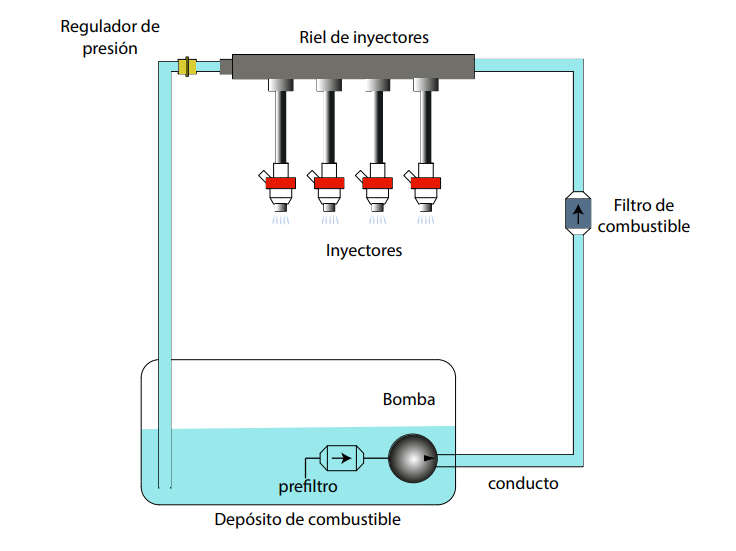
\includegraphics[width=0.9\textwidth]{Images/sistema.png}
	\vspace{0.2cm}
	
	% 3. La nota de la figura según APA 7 (Con descripción técnica)
	\begin{flushleft}
		\footnotesize \textit{Nota.} Disposición física y conectividad de los elementos constitutivos del sistema, incluyendo unidades de control, sensores de monitoreo de parámetros y actuadores para la dosificación de combustible. Elaboración propia con base en~\citep{Fundamentos_Inyeccion}.
	\end{flushleft}
\end{figure}
    
    
\subsubsection{Sensores}

Los sensores son dispositivos encargados de medir diferentes variables de funcionamiento del motor y enviar esta información a la ECU para que pueda calcular la cantidad exacta de combustible necesaria en cada condición de operación \citep{Bosch_Automotive, web_sensores_motor}.

Entre los sensores más importantes del sistema de inyección electrónica se encuentran:
\begin{itemize}
    \item Sensor MAF (\textit{Mass Air Flow}): mide el flujo de aire que ingresa al motor.
    \item Sensor MAP (\textit{Manifold Absolute Pressure}): mide la presión del múltiple de admisión.
    \item Sensor TPS (\textit{Throttle Position Sensor}): detecta la posición de la mariposa de aceleración.
    \item Sensor ECT (\textit{Engine Coolant Temperature}): mide la temperatura del refrigerante.
    \item Sensor de oxígeno o lambda: controla la cantidad de oxígeno presente en los gases de escape.
\end{itemize}

La información proporcionada por estos sensores permite que la ECU ajuste continuamente la mezcla aire-combustible, optimizando el rendimiento del motor y reduciendo emisiones contaminantes.


\subsection{Control de la mezcla aire-combustible}

El control de la mezcla aire-combustible constituye uno de los procesos fundamentales en los sistemas modernos de inyección electrónica, debido a su influencia directa sobre la eficiencia térmica del motor, el consumo de combustible y la formación de emisiones contaminantes durante la combustión \citep{Fundamentos_Inyeccion, Bosch_GDI}.

La mezcla aire-combustible se define como la proporción entre la masa de aire y la masa de combustible que ingresa al cilindro para llevar a cabo el proceso de combustión. En motores a gasolina, la relación estequiométrica ideal se aproxima a 14,7:1, es decir, 14,7 partes de aire por cada parte de combustible \citep{Bosch_Automotive}. Esta condición permite una combustión más eficiente y favorece el funcionamiento adecuado del convertidor catalítico.

Para evaluar la calidad de la mezcla, se utiliza el factor lambda ($\lambda$), definido como:

\begin{equation}
	\lambda = \frac{(A/F)_{\mathrm{real}}}{(A/F)_{\mathrm{estequiometrico}}}
	\label{eq:lambda}
\end{equation}

Donde $(A/F)_{\mathrm{real}}$ representa la relación aire-combustible presente en el motor y $(A/F)_{\mathrm{estequiometrico}}$ corresponde a la relación ideal para la combustión completa.

Las variaciones del factor lambda afectan de manera significativa tanto las emisiones contaminantes como el desempeño del motor. Las mezclas ricas incrementan la emisión de monóxido de carbono (CO) e hidrocarburos no quemados (HC), mientras que las mezclas pobres pueden favorecer la formación de óxidos de nitrógeno (NO$_x$) y provocar una disminución de la potencia entregada por el motor \citep{Combustion_Emissions_2020}.

El control de esta mezcla es realizado por la unidad de control electrónico (ECU), la cual recibe información de distintos sensores del motor para ajustar de forma continua el tiempo de inyección y mantener condiciones de combustión adecuadas. Entre los sensores más relevantes se encuentran el sensor MAF, el sensor MAP, el sensor TPS, el sensor ECT y, de manera especial, el sensor de oxígeno o sensor lambda, encargado de medir la concentración de oxígeno presente en los gases de escape \citep{Bosch_Automotive, Fundamentos_Inyeccion}.

A partir de la señal proporcionada por el sensor lambda, la ECU puede implementar un control en lazo cerrado (\textit{closed loop}), mediante el cual corrige de forma dinámica la cantidad de combustible inyectado para mantener el valor de $\lambda$ cercano a 1. Este mecanismo mejora la eficiencia del motor, reduce el consumo de combustible y contribuye a la disminución de las emisiones contaminantes \citep{Bosch_GDI}.

Finalmente, diversos estudios han demostrado que un control preciso de la mezcla aire-combustible tiene un impacto significativo en la reducción de emisiones vehiculares y en la optimización del desempeño energético de los motores de combustión interna. En este sentido, el desarrollo de estrategias avanzadas de control electrónico ha permitido mejorar el funcionamiento del motor bajo diferentes condiciones de carga, velocidad y operación \citep{Combustion_Emissions_2020}.

\subsection{Relación del sistema de inyección con el consumo de combustible}

El sistema de inyección electrónica tiene una relación directa con el consumo de combustible, debido a que la cantidad de combustible suministrada al motor depende del tiempo de apertura del inyector. En este contexto, la duración del pulso de inyección constituye una variable fundamental para estimar el consumo instantáneo, ya que representa el tiempo durante el cual el inyector permanece abierto y permite el paso del combustible hacia la cámara de combustión \citep{article2020fuelconsumption}.

De acuerdo con el artículo de referencia, el consumo instantáneo puede determinarse a partir de la medición de la duración del pulso de inyección, estableciéndose una correlación muy alta entre ambas variables, con un coeficiente de 0,99 \cite{article2020fuelconsumption}. Esto indica que, al incrementarse el ancho del pulso, aumenta también la cantidad de combustible inyectado; por el contrario, una reducción del tiempo de apertura disminuye el caudal de combustible y, en consecuencia, el consumo del motor \citep{article2020fuelconsumption}.

\begin{figure}[h]
	\centering
	
	% 1. El caption automático estilo APA 7 (Título conciso arriba)
	\caption{Relación entre el sistema de inyección y el consumo de combustible}
	\label{fig:sistema_inyeccion}
	\vspace{0.3cm}
	
	% 2. La imagen ajustada proporcionalmente al ancho del texto
	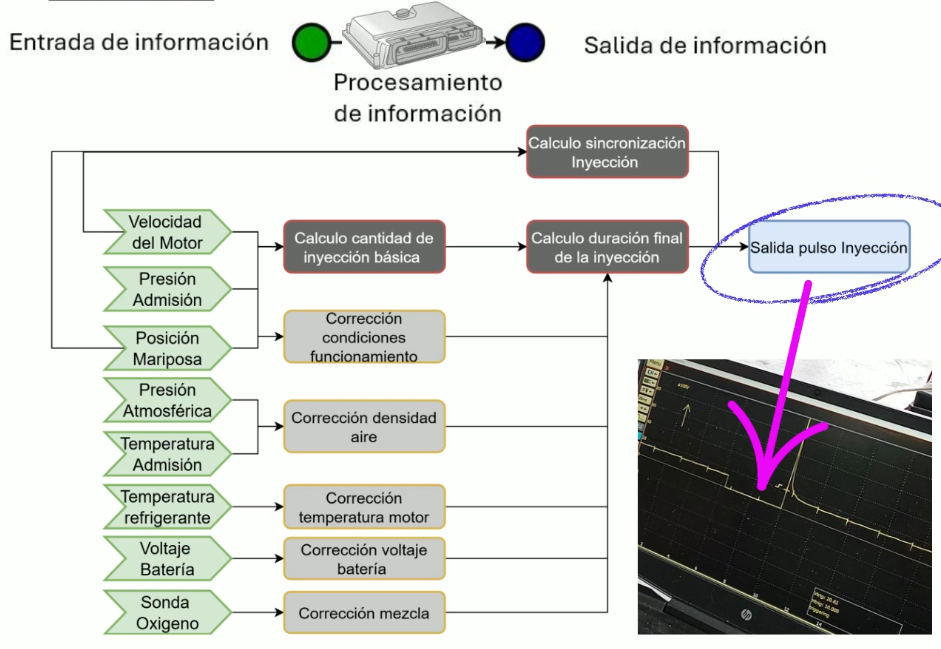
\includegraphics[width=0.9\textwidth]{Images/combu.png}
	\vspace{0.2cm}
	
	% 3. La nota de la figura según APA 7 (Con descripción técnica)
	\begin{flushleft}
		\footnotesize \textit{Nota.} Diagrama de bloques que ilustra cómo los parámetros medidos por la ECU (tiempo de inyección y flujo de masa de aire) impactan en el cálculo matemático del consumo instantáneo de combustible. Tomado de~\citep{Youtube_Inyeccion_2024}.
	\end{flushleft}
\end{figure}

La Figura \ref{fig:sistema_inyeccion} ilustra el proceso de adquisición y procesamiento de señales dentro del sistema de gestión del motor, donde las variables de entrada son procesadas por la unidad de control hasta generar la salida hacia el inyector. En particular, la señal de salida del pulso de inyección es el parámetro que permite regular la mezcla aire-combustible y, por tanto, influye de manera directa en el gasto de combustible durante la operación del motor \citep{article2020fuelconsumption}.

Por ello, el análisis del pulso de inyección resulta útil para estudiar el comportamiento real del motor bajo diferentes condiciones de operación, así como para evaluar estrategias orientadas a mejorar la eficiencia energética y reducir el consumo específico de combustible \citep{article2020fuelconsumption}.
%-------------------------2.6----------------
\section{Modelos matemáticos para el consumo del combustible}
\subsection{Concepto de consumo de combustible}

El consumo de combustible se define como la cantidad de combustible que utiliza un motor o vehículo para desarrollar un recorrido o mantener su operación durante un periodo determinado. Este parámetro constituye una de las variables más importantes en el análisis del desempeño automotriz, debido a que refleja de manera directa la eficiencia energética del sistema de propulsión y su impacto económico y ambiental \citep{PosadaHenao2016, EstimacionAlgoritmoUPS}.

Desde el punto de vista técnico, el consumo puede expresarse en términos de volumen o masa de combustible por unidad de distancia recorrida, como litros por cada 100 km (L/100 km), o por unidad de tiempo, como litros por hora (L/h), dependiendo del tipo de evaluación que se requiera \citep{PosadaHenao2016}. En motores de combustión interna, este indicador no solo depende de la demanda de potencia, sino también de las condiciones de operación del vehículo, tales como la velocidad, la carga, la pendiente del terreno, la resistencia aerodinámica y el estado del sistema de inyección \citep{ConsumoVehiculos2002, PosadaHenao2016}.

En términos generales, un menor consumo de combustible se asocia con una mejor eficiencia del motor, siempre que se mantengan condiciones adecuadas de potencia y funcionamiento. Sin embargo, este comportamiento puede variar en función de la estrategia de control del motor, la calidad de la combustión y las características del trayecto o ciclo de conducción \citep{EstimacionAlgoritmoUPS, ConsumoVehiculos2002}.

Por esta razón, el estudio del consumo de combustible constituye una base fundamental para el desarrollo de modelos matemáticos que permitan estimar, comparar y optimizar el desempeño de los motores en diferentes condiciones de operación \citep{PosadaHenao2016}.

\subsection{Métodos de estimación del consumo}

La estimación del consumo de combustible ha sido abordada mediante distintos enfoques matemáticos y experimentales, cuyo objetivo principal es determinar con precisión la cantidad de combustible utilizada por un vehículo durante su operación. En términos generales, estos métodos pueden clasificarse en modelos basados en variables de conducción, modelos fundamentados en parámetros del motor y modelos estadísticos o híbridos que combinan distintas señales del sistema vehicular \citep{EstimacionConsumoTransporte2004, EstimacionAlgoritmoUPS}.

Los modelos basados en variables de conducción utilizan información como la velocidad, la distancia recorrida, la aceleración y las condiciones de operación del vehículo para aproximar el consumo. Este tipo de enfoque resulta útil cuando no se dispone de acceso directo a variables internas del motor, aunque su precisión puede verse limitada por las variaciones propias del ciclo de conducción y por la topografía de la ruta \citep{ConsumoVehiculos2002, EstimacionConsumoTransporte2004}.

Por otro lado, los modelos basados en parámetros del motor emplean señales obtenidas desde la unidad de control electrónico o mediante el puerto OBD-II, tales como el flujo másico de aire (MAF), la posición del acelerador (TPS), las revoluciones por minuto (RPM) y la relación aire-combustible. Estos modelos presentan una mayor capacidad de representación del comportamiento real del motor, ya que incorporan variables directamente relacionadas con la formación de la mezcla y la entrega de combustible \citep{MAFFuelConsumption2024, ResearchOBD2018}.

Adicionalmente, existen métodos estadísticos y de aprendizaje automático que permiten construir relaciones empíricas entre variables de operación y consumo de combustible. Aunque estos enfoques pueden ofrecer buenos niveles de predicción, requieren bases de datos representativas y procesos de calibración adecuados para asegurar su validez en diferentes condiciones de uso \citep{EstimatingRegression2018, ResearchOBD2018}.

En este contexto en la Tabla \ref{tab:estim} se muestra, la selección del método de estimación depende de la disponibilidad de datos, el nivel de precisión requerido y la complejidad aceptable del modelo . Para aplicaciones en tiempo real, los modelos basados en sensores como el MAF representan una alternativa adecuada, debido a que permiten relacionar directamente la masa de aire admitida por el motor con la cantidad de combustible necesaria para mantener una combustión eficiente \citep{MAFFuelConsumption2024, Bosch_GDI}.

\begin{table}[h]
	\centering
	% Título separado bajo norma estricta APA 7
	\captionsetup{labelformat=simple, labelsep=newline, textfont=it, labelfont=bf}
	\caption{Comparación de métodos para la estimación del consumo de combustible}
	\label{tab:estim}
	\vspace{0.3cm}
	
	% Usamos tabularx para una distribución fluida y equilibrada de las columnas
	\begin{tabularx}{\linewidth}{p{2.5cm} X X X}
		\toprule % Línea superior APA 7
		\rowcolor[rgb]{0.851, 0.851, 0.851}
		\textbf{Método} & \textbf{Principio} & \textbf{Ventajas} & \textbf{Limitaciones} \\
		\midrule % Línea divisoria de encabezado APA 7
		Estadístico & Relaciona consumo con variables observables como velocidad o distancia. & Simple y económico. & Menor precisión en condiciones variables. \\
		\addlinespace
		Mecanicista & Usa fuerzas resistivas y demanda de potencia del vehículo. & Más físico y explicativo. & Requiere mayor cantidad de parámetros y calibración. \\
		\addlinespace
		Basado en sensores & Utiliza señales directas de la ECU como MAF, MAP, TPS o sonda lambda. & Ideal para la estimación y monitoreo en tiempo real. & Depende de la tasa de refresco y calidad de los sensores. \\
		\bottomrule % Línea inferior de cierre APA 7
	\end{tabularx}
	\vspace{0.2cm}
	
	\begin{flushleft}
		\footnotesize \textit{Nota.} Elaboración propia.
	\end{flushleft}
\end{table}

\subsection{Relación aire-combustible (AFR)}

La relación aire-combustible, conocida como \textit{Air-Fuel Ratio} (AFR), expresa la proporción existente entre la masa de aire y la masa de combustible que ingresan al cilindro durante el proceso de combustión. Este parámetro es fundamental en el análisis del funcionamiento de los motores de combustión interna, ya que determina la calidad de la mezcla y condiciona directamente la eficiencia térmica, el consumo de combustible y la generación de emisiones contaminantes \citep{AFRLambdaHPAcademy, AFRAnsed}.

En motores a gasolina, la relación estequiométrica de referencia es aproximadamente 14.7:1, lo que significa que se requieren 14.7 partes de aire por cada parte de combustible para lograr una combustión ideal \citep{AFRLambdaHPAcademy, Bosch_Automotive}. Bajo esta condición, el combustible puede oxidarse de manera más completa y se favorece el funcionamiento adecuado de los sistemas de postratamiento, como el convertidor catalítico.

Cuando la relación aire-combustible es inferior a la estequiométrica, la mezcla se considera rica, debido al exceso de combustible presente en la cámara de combustión. En este caso, aumenta la probabilidad de generar monóxido de carbono (CO) e hidrocarburos no quemados (HC), debido a una combustión incompleta \citep{AFRAnsed}. Por el contrario, cuando la relación aire-combustible es superior a la estequiométrica, la mezcla es pobre, lo que implica un exceso de aire. Esta condición puede disminuir el consumo de combustible, pero también puede afectar la potencia del motor y favorecer la formación de óxidos de nitrógeno (NO$_x$) \citep{AFRLambdaHPAcademy, Combustion_Emissions_2020}.

\begin{figure}[h]
	\centering
	
	% 1. El caption automático estilo APA 7 (Título conciso arriba)
	\caption{Curva estequiométrica del factor lambda y respuesta del sensor de oxígeno}
	\label{fig:factor_lambda}
	\vspace{0.3cm}
	
	% 2. La imagen ajustada proporcionalmente al ancho del texto
	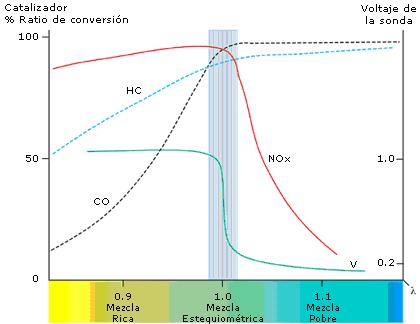
\includegraphics[width=0.75\textwidth]{Images/Sonda.JPG}
	\vspace{0.2cm}
	
	% 3. La nota de la figura según APA 7 (Con descripción técnica)
	\begin{flushleft}
		\footnotesize \textit{Nota.} Comportamiento de la señal de voltaje generada por el sensor de oxígeno en función del factor lambda, detallando las regiones de transición entre mezcla rica y mezcla pobre. Adaptado de~\citep{Fundamentos_Inyeccion}.
	\end{flushleft}
\end{figure}

La AFR está estrechamente relacionada con el factor lambda ($\lambda$), el cual permite expresar qué tan lejos se encuentra la mezcla real respecto de la condición estequiométrica ver Tabla \ref{tab:afr} En términos generales, el control de la AFR constituye una estrategia esencial para mantener una combustión eficiente y adaptar la entrega de combustible a las condiciones de carga, velocidad y demanda del motor \citep{Bosch_GDI, Fundamentos_Inyeccion}.

Para el cálculo final del consumo, es fundamental definir la relación aire-combustible ($AFR$), la cual se expresa como la proporción entre la masa de aire y la masa de combustible:

\begin{equation}
	AFR = \frac{m_{aire}}{m_{combustible}}
\end{equation}

En los sistemas de gestión modernos, esta relación se normaliza mediante el factor $\lambda$ (lambda), que relaciona el $AFR$ real medido por la sonda de oxígeno con el valor estequiométrico ideal:

\begin{equation}
	\lambda = \frac{AFR_{real}}{AFR_{estequiometrico}}
\end{equation}

Si $\lambda = 1$, la mezcla es estequiométrica; si $\lambda < 1$, la mezcla es rica (exceso de combustible), y si $\lambda > 1$, la mezcla es pobre (exceso de aire) ver Figura \ref{fig:factor_lambda}.

Por esta razón, el análisis de la relación aire-combustible es indispensable dentro de los modelos matemáticos de estimación del consumo de combustible, ya que permite vincular la cantidad de aire admitida con la masa de combustible requerida para sostener una operación eficiente del motor.

\begin{table}[htbp]
	\centering
	% Título separado bajo norma estricta APA 7
	\captionsetup{labelformat=simple, labelsep=newline, textfont=it, labelfont=bf}
	\caption{Interpretación de la relación aire-combustible y el factor lambda}
	\label{tab:afr}
	\vspace{0.3cm}
	
	% Usamos tabularx para un autoajuste milimétrico a los márgenes
	\begin{tabularx}{\linewidth}{p{3.8cm} p{2.8cm} p{2.2cm} X}
		\toprule % Línea superior APA 7
		\rowcolor[rgb]{0.851, 0.851, 0.851}
		\textbf{Condición} & \textbf{Relación AFR} & \textbf{Factor $\lambda$} & \textbf{Efecto principal y aplicación} \\
		\midrule % Línea divisoria de encabezado APA 7
		\textbf{Mezcla rica} & AFR $<$ 14,7:1 & $\lambda < 1$ & Mayor consumo de combustible y aumento de emisiones de CO y HC. Típica en aceleraciones a plena carga. \\
		\addlinespace
		\textbf{Mezcla estequiométrica} & AFR = 14,7:1 & $\lambda = 1$ & Combustión completa y eficiente, operación óptima del catalizador. Condición ideal de crucero. \\
		\addlinespace
		\textbf{Mezcla pobre} & AFR $>$ 14,7:1 & $\lambda > 1$ & Menor consumo de combustible, incremento de temperatura en la cámara y emisiones de NOx. \\
		\bottomrule % Línea inferior de cierre APA 7
	\end{tabularx}
	\vspace{0.2cm}
	
	\begin{flushleft}
		\footnotesize \textit{Nota.} Comportamiento físico-químico de la dosificación de la mezcla aire-combustible en motores de gasolina y su impacto en la eficiencia y emisiones. Elaboración propia.
	\end{flushleft}
\end{table}

\subsection{Modelo basado en el sensor MAF}

El sensor MAF (\textit{Mass Air Flow}) es uno de los sensores más importantes dentro de los sistemas modernos de inyección electrónica, debido a que permite medir la cantidad de aire que ingresa al motor. Esta información es utilizada por la unidad de control electrónico (ECU) para calcular la cantidad adecuada de combustible necesaria para mantener una combustión eficiente \citep{Bosch_Automotive, Fundamentos_Inyeccion}. 

El funcionamiento del sensor MAF se basa generalmente en el principio de hilo caliente (\textit{Hot Wire}). En este sistema, un filamento metálico es calentado eléctricamente a una temperatura constante. Cuando el aire atraviesa el conducto de admisión, enfría el filamento y provoca una variación en la corriente eléctrica necesaria para mantener la temperatura estable. La ECU interpreta esta variación como una medida del flujo de aire que entra al motor \citep{Hella_MAF, Bosch_GDI}.

La información proporcionada por el sensor MAF permite mejorar el control de la mezcla aire–combustible, optimizar el consumo de combustible y reducir emisiones contaminantes. Además, este sensor es ampliamente utilizado en estrategias de monitoreo y diagnóstico automotriz debido a que el flujo de aire está directamente relacionado con la cantidad de combustible consumida por el motor \citep{Fundamentos_Inyeccion}.

La Figura \ref{fig:maf_sensor} muestra la ubicación típica y el principio de funcionamiento de un sensor MAF dentro del sistema de admisión del motor.

\begin{figure}[h]
	\centering
	
	% 1. El caption automático estilo APA 7 (Título descriptivo arriba)
	\caption{Principio de funcionamiento eléctrico y térmico del sensor MAF}
	\label{fig:maf_sensor}
	\vspace{0.3cm}
	
	% 2. La imagen ajustada proporcionalmente al ancho del texto
	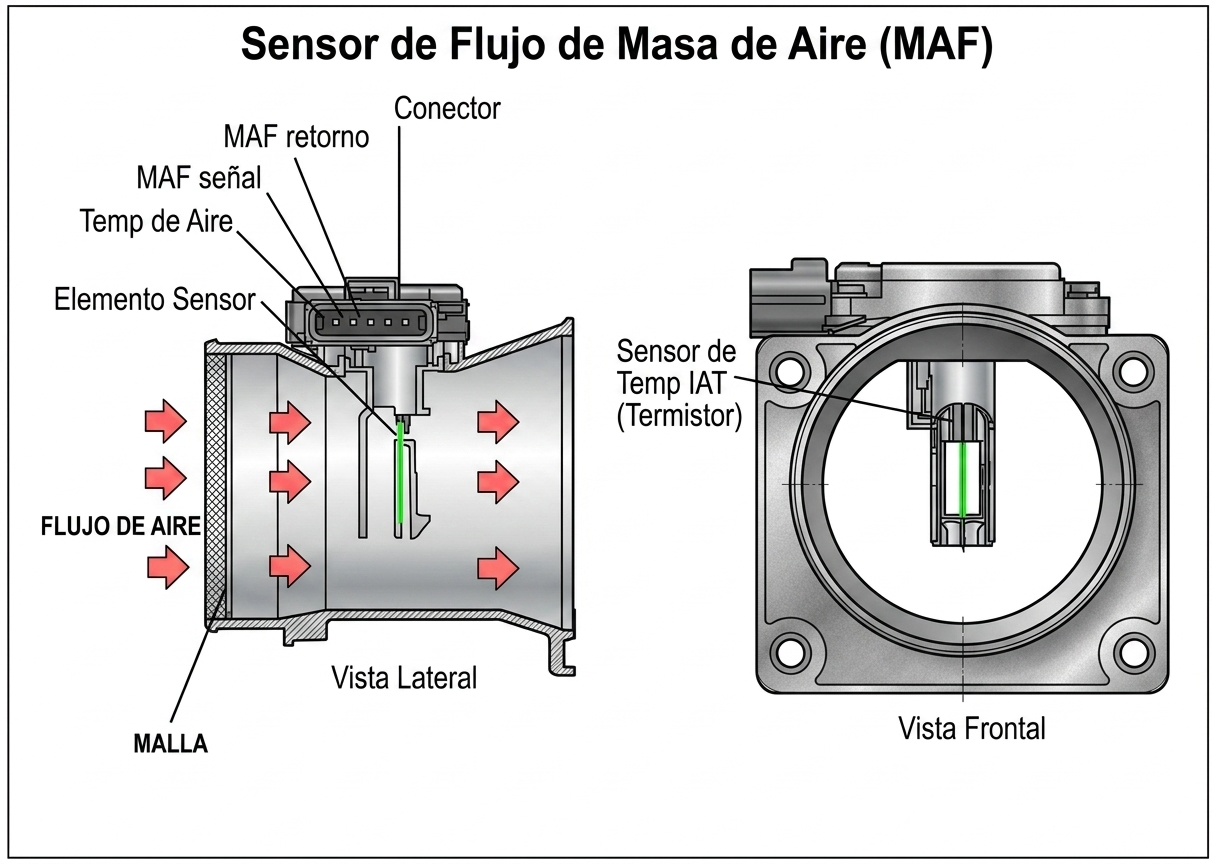
\includegraphics[width=0.75\textwidth]{Images/maf_sensor.png}
	\vspace{0.2cm}
	
	% 3. La nota de la figura según APA 7 (Con descripción técnica)
	\begin{flushleft}
		\footnotesize \textit{Nota.} Diagrama del comportamiento del flujo de masa de aire sobre el elemento térmico (hilo caliente), ilustrando cómo la transferencia de calor altera la resistencia eléctrica y la señal de salida hacia la ECU. Adaptado de~\citep{Hella_MAF}.
	\end{flushleft}
\end{figure}


Uno de los métodos más utilizados para estimar el consumo de combustible en tiempo real consiste en emplear directamente la señal del sensor MAF. Este enfoque se basa en la relación estequiométrica aire–combustible, considerando que para motores a gasolina la mezcla ideal es aproximadamente 14,7:1 \citep{Bosch_Automotive}.

El consumo de combustible puede calcularse mediante la siguiente expresión:

\begin{equation}
	FuelConsumption_{(L/h)} = \frac{MAF_{(g/s)} \times 3600}{14.7 \times 745}
\end{equation}

En esta expresión, los valores constantes representan:
\begin{itemize}
	\item \textbf{3600}: Factor de conversión de segundos a horas.
	\item \textbf{14.7}: Relación aire-combustible estequiométrica ideal para la gasolina.
	\item \textbf{745}: Densidad aproximada de la gasolina en $g/L$ (este valor puede oscilar entre $720$ y $775$ $g/L$ según la temperatura y el octanaje).
\end{itemize}

donde:

Para el cálculo operativo en motores a gasolina, se asumen valores estándar que permiten simplificar la monitorización en tiempo real. En este modelo, se consideran las siguientes constantes:

\begin{equation}
	AFR_{estequiometrico} = 14.7
\end{equation}

\begin{equation}
	\rho_{fuel} \approx 750 \, \mathrm{g/L}
\end{equation}

Es importante destacar que la densidad de la gasolina es una variable sensible a la composición química, el porcentaje de aditivos y las condiciones ambientales. En el contexto de \textbf{Bolivia}, la gasolina comercial incorpora mezclas de bioetanol (como la Gasolina Especial Plus o la Súper Etanol), lo que puede generar variaciones en la densidad y en el poder calorífico respecto a las gasolinas convencionales puras \citep{ANH_Gasolina_87}.

Sustituyendo estos valores en la fórmula general, la ecuación de consumo instantáneo se simplifica mediante un factor de conversión aproximado:

\begin{equation}
	FuelConsumption_{(L/h)} \approx MAF_{(g/s)} \times 0.33
\end{equation}

\subsection{Ejemplo de Cálculo Instantáneo}

Para ilustrar la sensibilidad del modelo, se propone el siguiente escenario: si el sistema (vía sensores MAP+IAT o MAF) registra un flujo de masa de aire de $10 \, g/s$, el consumo instantáneo se calcula como:

\begin{equation}
	FuelConsumption = \frac{10 \times 3600}{14.7 \times 745}
\end{equation}

\begin{equation}
	FuelConsumption \approx 3.29 \, \mathrm{L/h}
\end{equation}

Este resultado permite al sistema de gestión o al usuario final visualizar el gasto volumétrico de combustible en función de la carga del motor en un momento determinado.

Este modelo permite obtener estimaciones relativamente precisas del consumo instantáneo de combustible utilizando únicamente información proveniente del sistema OBD-II. Debido a su simplicidad y facilidad de implementación, es ampliamente utilizado en aplicaciones de telemetría, monitoreo vehicular y análisis de eficiencia energética \citep{CSSElectronics_OBD2, Hella_MAF}.

En el presente proyecto, este modelo constituye una de las principales estrategias para estimar el consumo de combustible en tiempo real mediante la adquisición de datos desde la ECU del vehículo a través del protocolo OBD-II.


\subsection{El Método Speed-Density: Origen y Evolución}

El modelo basado en los sensores MAP e IAT es técnicamente denominado el método \textbf{Speed-Density} (Velocidad-Densidad). Recibe este nombre porque el flujo de masa de aire no se mide directamente, sino que se infiere a partir de la \textit{velocidad} del motor (RPM) y la \textit{densidad} del aire en el colector de admisión.


Aunque el concepto de densidad de gases se remonta a la termodinámica clásica, su aplicación en el control electrónico de motores (ECU) fue impulsada por la necesidad de cumplir con las normativas de emisiones contaminantes en la década de 1970.

Uno de los pioneros en la implementación masiva de sistemas electrónicos basados en presión de vacío fue la compañía Bendix Corporation con su sistema Electrojector, y posteriormente Bosch con el sistema D-Jetronic(donde la "D" proviene del alemán Druck, que significa presión).

Este sistema fue revolucionario porque reemplazó los carburadores mecánicos por una unidad de control analógica que leía la presión del colector (MAP) para determinar el pulso de inyección. A diferencia del sistema \textit{L-Jetronic} (que usa flujo de aire directo o MAF), el sistema \textit{D-Jetronic} sentó las bases del algoritmo Speed-Density moderno.

El nombre deriva directamente de las dos variables fundamentales que la computadora del motor utiliza para consultar sus mapas de combustible:

\begin{enumerate}
	\item \textbf{Speed (Velocidad):} Se refiere a la velocidad angular del motor ($N$ en RPM). Esta variable determina la frecuencia con la que los cilindros "bombean" aire hacia adentro.
	\item \textbf{Density (Densidad):} Calculada mediante la presión (MAP) y la temperatura (IAT). La densidad ($\rho$) nos dice cuánta masa de aire hay en un volumen determinado de espacio en el colector.
\end{enumerate}

La relación fundamental del método establece que la masa de aire por cilindro ($m_{cyl}$) es proporcional a la densidad del aire en el colector multiplicada por el volumen del cilindro y corregida por la eficiencia volumétrica:

\begin{equation}
	m_{cyl} = \eta_v(N, P) \cdot \rho_{intake} \cdot V_{cyl}
\end{equation}


El uso de Speed-Density sobre otros métodos (como MAF) tiene implicaciones técnicas importantes:

\begin{itemize}
	\item \textbf{Robustez Mecánica:} Los sensores MAP son extremadamente duraderos y no obstruyen el flujo de aire, a diferencia de los hilos calientes de los sensores MAF que pueden ensuciarse.
	\item \textbf{Respuesta Transitoria:} En motores con turbocompresores de alto rendimiento, el método Speed-Density suele ser más rápido para reaccionar a cambios súbitos de presión.
	\item \textbf{Dependencia de la Calibración:} La mayor desventaja es que el sistema "no sabe" si el motor ha sido modificado (por ejemplo, levas más agresivas). Cualquier cambio físico requiere recalibrar la tabla de eficiencia volumétrica ($\eta_v$) en la ECU, ya que el cálculo es puramente matemático y no una medición física directa del aire.
\end{itemize}



\subsection{Densidad del combustible}

La densidad del combustible es una propiedad física que relaciona la masa de un fluido con el volumen que ocupa. En el caso de los combustibles líquidos, esta magnitud es relevante porque influye en la energía contenida por unidad de volumen, en el caudal inyectado y en la estimación del consumo de combustible. Por esta razón, en los ensayos de calidad de carburantes se suele reportar la densidad en condiciones normalizadas de temperatura, generalmente a 15,6$^\circ$C o 20$^\circ$C, con el fin de garantizar la comparabilidad de los resultados \citep{ANH2014, FuelsDensityToolbox}.

A nivel del mar y en condiciones normalizadas de laboratorio, la densidad de la gasolina suele ubicarse aproximadamente entre 0,71 y 0,78 g/cm$^3$, mientras que en el diésel se encuentra en un rango aproximado de 0,82 a 0,85 g/cm$^3$, aunque estos valores pueden variar según la formulación, los aditivos y la temperatura de medición \citep{FuelsDensityToolbox}. En consecuencia, una misma masa de combustible puede ocupar distinto volumen dependiendo de su densidad, lo cual afecta la forma en que se expresa y compara el consumo en términos volumétricos.

En la práctica, la densidad del combustible disminuye cuando aumenta la temperatura, debido a la expansión térmica del líquido. Por ello, los organismos técnicos y las normas de control de calidad establecen valores de referencia y métodos estandarizados de medición, como D-1298 y D-4052, para asegurar que los resultados no dependan de variaciones ambientales durante el ensayo \citep{ANH2014}.

En la ciudad de La Paz, Bolivia, la evaluación de combustibles debe considerarse dentro de un contexto de altitud elevada, cercana a 3600 m. s. n. m., donde la presión atmosférica es menor que a nivel del mar \citep{BarometricaPaz}. Aunque la densidad del combustible como propiedad intrínseca no depende directamente de la altitud, las condiciones ambientales de operación del motor sí influyen en el comportamiento de la combustión y en la estimación real del consumo, por lo que resulta necesario trabajar con valores corregidos o medidos bajo condiciones controladas \citep{ANH2014}.

En la Tabla \ref{tab:densidad} se presenta valores aproximados de algunos carburantes utilizados en sistemas de combustión interna.


\begin{table}[h]
	\centering
	% Título separado bajo norma estricta APA 7
	\captionsetup{labelformat=simple, labelsep=newline, textfont=it, labelfont=bf}
	\caption{Densidad típica de combustibles líquidos a temperatura de referencia}
	\label{tab:densidad}
	\vspace{0.3cm}
	
	% Usamos tabularx para una distribución fluida y adaptativa
	\begin{tabularx}{\linewidth}{p{3.5cm} p{4.5cm} X}
		\toprule % Línea superior APA 7
		\rowcolor[rgb]{0.851, 0.851, 0.851}
		\textbf{Combustible} & \textbf{Densidad aproximada} & \textbf{Observación} \\
		\midrule % Línea divisoria de encabezado APA 7
		Gasolina & 0,715 -- 0,780 g/cm$^{3}$ & Varía según la formulación estacional y la temperatura. \\
		\addlinespace
		Diésel & 0,820 -- 0,845 g/cm$^{3}$ & Presenta mayor densidad y contenido energético que la gasolina. \\
		\addlinespace
		Jet fuel & 0,775 -- 0,840 g/cm$^{3}$ & Sujeto a especificaciones y normativas internacionales aeronáuticas. \\
		\addlinespace
		GLP & Variable & Altamente dependiente de la proporción de la mezcla propano-butano. \\
		\bottomrule % Línea inferior de cierre APA 7
	\end{tabularx}
	\vspace{0.2cm}
	
	\begin{flushleft}
		\footnotesize \textit{Nota.} Valores de referencia utilizados para la conversión volumétrica en el cálculo de tasas de consumo masivo en sistemas de combustión interna. Elaboración propia.
	\end{flushleft}
\end{table}

En este sentido, la densidad del combustible constituye una variable de apoyo dentro de los modelos matemáticos de consumo, especialmente cuando se desea convertir el caudal volumétrico a caudal másico o cuando se analizan diferencias de desempeño entre distintas zonas geográficas.

\subsection{Efecto de la altura en el consumo de gasolina}

La altura sobre el nivel del mar influye de manera significativa en el desempeño de los motores de combustión interna, debido a que al aumentar la altitud disminuyen la presión atmosférica y la densidad del aire. Esta reducción implica una menor cantidad de oxígeno disponible por unidad de volumen, lo que afecta directamente el proceso de combustión y la potencia desarrollada por el motor \citep{LopezRuano2018}.

En motores de aspiración natural, la disminución de la presión barométrica reduce la masa de aire que ingresa al cilindro durante la carrera de admisión. Como consecuencia, la ECU debe modificar la cantidad de combustible inyectado para conservar una relación aire-combustible adecuada. Si esta compensación no es suficiente, la combustión puede volverse menos eficiente y el consumo específico de combustible puede incrementarse, especialmente en condiciones de carga elevada o conducción exigente \citep{LopezRuano2018}.

Diversos estudios indican que, como referencia práctica, la potencia de un motor atmosférico puede disminuir aproximadamente un 10\% por cada 1\,000 m de incremento en la altitud, debido a la menor densidad del aire y a la reducción del oxígeno disponible para la combustión \citep{LopezRuano2018}. Sin embargo, el efecto sobre el consumo de gasolina no siempre es lineal, ya que también intervienen la estrategia de inyección, la aerodinámica del vehículo, la topografía del recorrido y el estilo de conducción.

En la ciudad de La Paz, ubicada a gran altitud, esta condición tiene especial relevancia en el comportamiento de los vehículos con motor de gasolina. A menor presión atmosférica, el motor recibe una masa de aire menor en cada ciclo, por lo que el sistema de inyección debe ajustar la entrega de combustible para evitar mezclas excesivamente ricas o pobres. En consecuencia, el análisis del consumo en esta ciudad debe considerar no solo el volumen de combustible utilizado, sino también el contexto altitudinal y las condiciones de operación del vehículo \citep{LopezRuano2018, ANH2014} ver Tabla \ref{tab:altitud}.

Por ello, la altitud debe entenderse como una variable ambiental que modifica el rendimiento del motor y condiciona la estimación del consumo de gasolina, especialmente en vehículos no sobrealimentados y en trayectos urbanos donde las variaciones de carga y velocidad son frecuentes .

\begin{table}[h]
	\centering
	% Título separado bajo norma estricta APA 7
	\captionsetup{labelformat=simple, labelsep=newline, textfont=it, labelfont=bf}
	\caption{Efecto de la altitud sobre los parámetros del motor y el consumo de gasolina}
	\label{tab:altitud}
	\vspace{0.3cm}
	
	% Usamos tabularx para una distribución fluida y adaptativa entre los márgenes
	\begin{tabularx}{\linewidth}{p{3.0cm} X X}
		\toprule % Línea superior APA 7
		\rowcolor[rgb]{0.851, 0.851, 0.851}
		\textbf{Condición} & \textbf{Efecto físico} & \textbf{Consecuencia en el consumo} \\
		\midrule % Línea divisoria de encabezado APA 7
		Nivel del mar & Mayor presión barométrica y alta densidad del aire. & Combustión más estable y un óptimo llenado volumétrico del cilindro. \\
		\addlinespace
		Altitud media & Menor densidad del aire y reducción moderada en la concentración de oxígeno. & Ajustes dinámicos en los tiempos de inyección y variación del consumo nominal. \\
		\addlinespace
		Alta altitud & Reducción significativa de la presión barométrica y densidad atmosférica. & Pérdida de potencia efectiva (pérdida por bombeo) y potencial incremento del consumo específico. \\
		\bottomrule % Línea inferior de cierre APA 7
	\end{tabularx}
	\vspace{0.2cm}
	
	\begin{flushleft}
		\footnotesize \textit{Nota.} Relación termodinámica general entre la altitud geográfica, la densidad del aire de admisión y el comportamiento del consumo de combustible en motores de combustión interna atmosféricos. Elaboración propia.
	\end{flushleft}
\end{table}

%-------------------------2.7----------------
\section{Vehículos bi-fuel}

\subsection{Principio de funcionamiento}

Los vehículos bi-fuel o bicombustibles son aquellos cuyo sistema de propulsión está diseñado para operar con dos combustibles distintos, normalmente gasolina y un combustible gaseoso como GLP o GNV. Este tipo de configuración permite que el motor funcione con uno u otro combustible según las condiciones de operación, la disponibilidad energética y la estrategia de control implementada en la unidad electrónica del vehículo \citep{BifuelMotor1, BifuelMotorES, GasNaturalGNU}.

En términos generales, el motor bi-fuel conserva un único sistema de combustión, pero incorpora un conjunto adicional de componentes para la gestión del segundo combustible, tales como tanque, válvulas, regulador, inyectores y elementos de conmutación ver Figura \ref{fig:bifuel_sistema1}. El arranque suele realizarse con gasolina y, una vez alcanzadas ciertas condiciones de temperatura o funcionamiento, el sistema puede cambiar automáticamente al combustible alternativo \citep{DRBifuel, BifuelMotorES}.

\subsection{Tipos de combustibles utilizados}

Los combustibles más comunes en los vehículos bi-fuel son la gasolina y el gas licuado de petróleo (GLP) o el gas natural vehicular (GNV). También existen aplicaciones con biocombustibles y mezclas de combustibles fósiles y alternativos, aunque en el contexto vehicular el término bi-fuel se asocia principalmente al uso de gasolina combinada con GLP o GNV \citep{TiposCombustiblesWebfleet, BifuelMotor1}.

\begin{figure}[h]
	\centering
	
	% 1. El caption automático estilo APA 7 (Título descriptivo arriba)
	\caption{Esquema de componentes y distribución en una adaptación de sistema Bi-Fuel (Gasolina/GLP)}
	\label{fig:bifuel_sistema1}
	\vspace{0.3cm}
	
	% 2. La imagen ajustada proporcionalmente para mantener simetría visual
	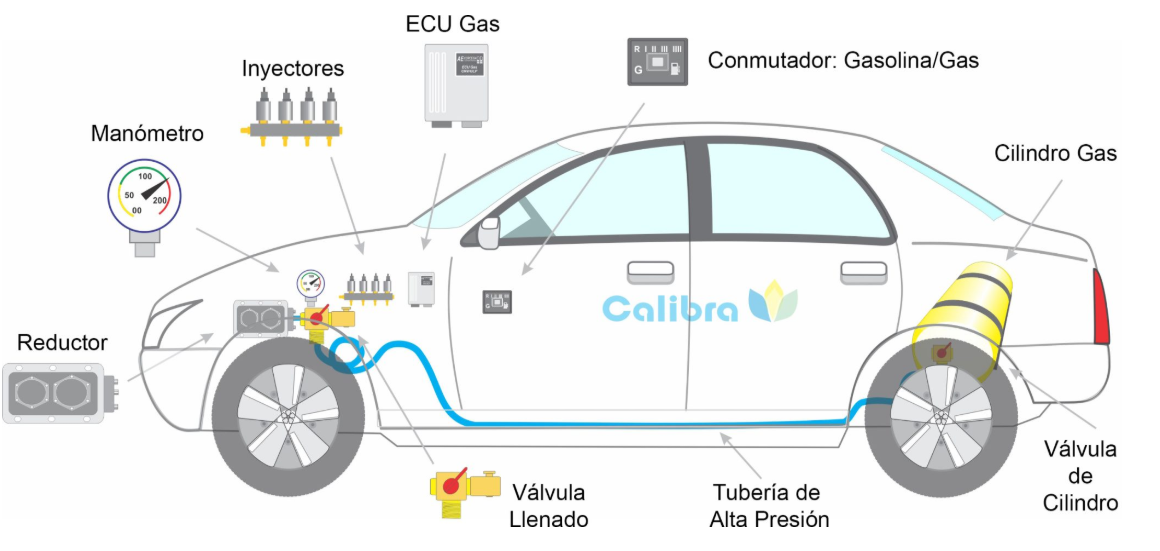
\includegraphics[width=0.95\textwidth]{Images/GLP.png}
	\vspace{0.2cm}
	
	% 3. La nota de la figura según APA 7 (Con descripción técnica)
	\begin{flushleft}
		\footnotesize \textit{Nota.} Arquitectura de instalación y flujo de señales en un motor adaptado para doble combustible, detallando la integración de la ECU secundaria de gas, el regulador de presión, la rampa de inyectores de GLP y el tanque de almacenamiento con su respectiva multivalvula. Adaptado de~\citep{GasNaturalGNU}.
	\end{flushleft}
\end{figure}

La elección del combustible alternativo depende de factores como la infraestructura disponible, el costo por unidad de energía, la autonomía requerida y la compatibilidad del sistema de inyección y encendido con las características del combustible \citep{GasNaturalGNU, BifuelMotor1}.

\subsection{Ventajas y desventajas}

Entre las principales ventajas de los vehículos bi-fuel se encuentra la posibilidad de extender la autonomía del vehículo al disponer de dos sistemas de alimentación, así como la reducción del costo operativo cuando se utiliza el combustible alternativo. Además, el uso de GLP o GNV suele asociarse con menores emisiones de CO$_2$ y NO$_x$, lo cual representa una ventaja ambiental frente al uso exclusivo de gasolina \citep{ GasNaturalGNU, Fedebiocombustibles}.

No obstante, este tipo de tecnología también presenta desventajas. En algunos casos, el motor puede experimentar una ligera reducción de potencia cuando opera con el combustible alternativo, especialmente en configuraciones a GLP. Asimismo, la instalación del sistema bi-fuel implica una mayor complejidad mecánica, costos iniciales más elevados y la necesidad de mantenimiento especializado \citep{ BifuelMotorES}.

\subsection{Impacto en el consumo de combustible}

El impacto de los vehículos bi-fuel sobre el consumo de combustible debe analizarse considerando que cada combustible posee una densidad energética distinta. En general, el consumo volumétrico con GLP o GNV puede ser mayor que con gasolina, aunque el costo por kilómetro recorrido puede disminuir debido al menor precio del combustible alternativo \citep{DRBifuel}.

En la práctica, la comparación del consumo debe realizarse en términos equivalentes de energía o costo operativo, ya que un mayor volumen consumido no necesariamente implica un mayor gasto económico. Por esta razón, los vehículos bi-fuel constituyen una alternativa interesante para aplicaciones donde se busca reducir el costo de operación y las emisiones, manteniendo la posibilidad de usar gasolina como respaldo energético \citep{GasNaturalGNU, BifuelMotorES}.

La Figura \ref{fig:bifuel_sistema2} puede utilizarse para mostrar la arquitectura general de un sistema bi-fuel, incluyendo los componentes principales del circuito de gasolina y del circuito de gas. Y seguidamente en la Tabla \ref{tab:bifuel} su comparación con diferentes combustibles.

\begin{figure}[h]
	\centering
	
	% 1. El caption automático estilo APA 7 (Título descriptivo arriba)
	\caption{Esquema de componentes que conforman un vehículo bi-fuel, mostrando la coexistencia de sistemas de inyección paralelos y su gestión electrónica integrada}
	\label{fig:bifuel_sistema2}
	\vspace{0.3cm}
	
	% 2. La imagen ajustada proporcionalmente para mantener simetría visual
	% Nota: Se redujo levemente a 0.95\textwidth para evitar desbordes accidentales
	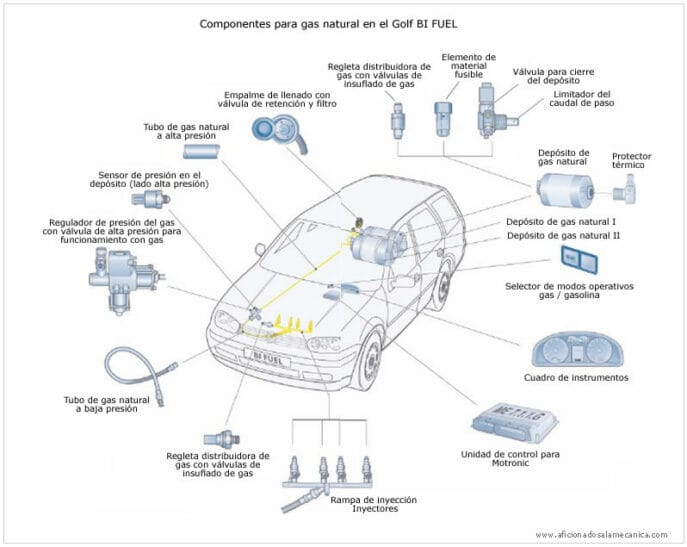
\includegraphics[width=0.95\textwidth]{Images/esquema-inyeccion-golf.jpg}
	\vspace{0.2cm}
	
	% 3. La nota de la figura según APA 7 (Con descripción técnica)
	\begin{flushleft}
		\footnotesize \textit{Nota.} Diagrama de bloques que ilustra la arquitectura de un motor adaptado para doble combustible (Gasolina/Gas). Se detalla la integración de la ECU secundaria, el regulador de presión, la rampa de inyectores de gas y el tanque de almacenamiento con su multivalvula, operando en paralelo al sistema de inyección original. Elaboración propia con base en~\citep{BifuelMotorES}.
	\end{flushleft}
\end{figure}

\begin{table}[h]
	\centering
	% Título separado bajo norma estricta APA 7
	\captionsetup{labelformat=simple, labelsep=newline, textfont=it, labelfont=bf}
	\caption{Comparación general entre combustibles en vehículos bi-fuel}
	\label{tab:bifuel}
	\vspace{0.3cm}
	
	% Usamos tabularx para una distribución fluida y adaptativa entre los márgenes
	\begin{tabularx}{\linewidth}{p{2.8cm} X X X}
		\toprule % Línea superior APA 7
		\rowcolor[rgb]{0.851, 0.851, 0.851}
		\textbf{Combustible} & \textbf{Ventaja principal} & \textbf{Limitación principal} & \textbf{Uso típico} \\
		\midrule % Línea divisoria de encabezado APA 7
		Gasolina & Mayor disponibilidad y arranque confiable en frío. & Mayor costo operativo y mayores emisiones de CO. & Operación principal o combustible de respaldo. \\
		\addlinespace
		GLP & Menor costo por kilómetro y reducción de emisiones. & Ligera pérdida de potencia y mayor consumo volumétrico. & Uso alternativo en vehículos convencionales adaptados. \\
		\addlinespace
		GNV & Alto rendimiento energético y bajas emisiones contaminantes. & Infraestructura de carga limitada y peso del tanque de almacenamiento. & Transporte urbano, flotas comerciales y transporte pesado. \\
		\bottomrule % Línea inferior de cierre APA 7
	\end{tabularx}
	\vspace{0.2cm}
	
	\begin{flushleft}
		\footnotesize \textit{Nota.} Comparación de parámetros operativos, económicos y logísticos de los combustibles más utilizados en vehículos dotados con sistemas de conversión de doble combustible. Elaboración propia.
	\end{flushleft}
\end{table}


%-------------------------2.9----------------
\section{Microcontroladores y sistemas embebidos}


\subsection{Microprocesador vs microcontrolador}
Un \textit{microprocesador} es un circuito integrado que contiene únicamente la unidad central de procesamiento (CPU), encargada de ejecutar instrucciones y procesar datos. Su función principal consiste en interpretar operaciones almacenadas en memoria externa, realizar cálculos aritméticos y lógicos y coordinar la ejecución de un programa mediante señales de control y buses de datos, direcciones e instrucciones .

A diferencia de otros dispositivos, el microprocesador por sí solo no forma un sistema funcional completo, ya que requiere memoria externa (RAM, ROM/Flash), periféricos de entrada/salida y circuitos auxiliares para operar en una aplicación real. Por esta razón, suele emplearse en sistemas de propósito general o en plataformas que demandan mayor capacidad de cómputo y flexibilidad, como computadoras de escritorio o sistemas de infoentretenimiento de alto nivel \citep{ MikroE2018}.

En contraste, un \textit{microcontrolador} integra en un solo chip la CPU, memoria (programa y datos) y periféricos de entrada y salida necesarios para ejecutar tareas específicas. Esta integración permite construir sistemas compactos, de bajo consumo y bajo costo, orientados a aplicación de control en tiempo real, como la gestión de sensores, actuadores y buses de comunicación. En el ámbito automotriz, los microcontroladores son ampliamente utilizados en unidades de control electrónico (ECU) para funciones de powertrain, chasis, seguridad y confort \citep{ EmbebidosUruguay}.

\subsection{Sistema embebido}
Un \textit{sistema embebido} es un sistema de cómputo diseñado para realizar una función específica dentro de un dispositivo o equipo mayor, en lugar de servir como plataforma de propósito general. Está compuesto por hardware (microcontrolador o microprocesador, sensores, actuadores, conversiones de señal, etc.), software (firmware o RTOS) y, en algunos casos, elementos mecánicos, con restricciones propias de tiempo, consumo energético y recursos disponibles \citep{EmbebidosUruguay, ITESOEmbebidos}.

Estos sistemas interactúan con el entorno físico mediante sensores y actuadores, y suelen operar en tiempo real o con tiempos de respuesta acotados. Debido a su naturaleza específica, se optimizan para resolver una tarea concreta (por ejemplo, medir el flujo de combustible, controlar el encendido o gestionar una bomba eléctrica) con alta confiabilidad, bajo costo y consumo reducido de energía. En la industria automotriz, prácticamente todas las ECUs presentes en el vehículo constituyen sistemas embebidos \citep{EmbebidosUruguay, AutomotiveEmbeddedHandbook}.

\subsection{Arquitectura de microcontroladores}

Como se ha señalado, un \textit{microcontrolador} combina núcleo, memoria RAM y periféricos. Con el fin de profundizar en su funcionamiento, en esta sección se describirán teóricamente estos elementos y se analizarán las arquitecturas que definen su estructura.

\subsubsection{Núcleo/CPU}
El núcleo o CPU de un microcontrolador es el bloque encargado de ejecutar las instrucciones del programa, gestionar registros internos y controlar el flujo de datos entre los distintos componentes del sistema. En la actualidad, los microcontroladores más utilizados en aplicaciones automotrices se basan en arquitecturas de tipo RISC, como los núcleos ARM Cortex‑M, AVR o PIC , que ofrecen un buen equilibrio entre rendimiento, consumo energético y facilidad de programación \citep{MikroE2018}.

Estos últimos se detallan en la Tabla \ref{tab:arqui}

\begin{table}[htbp]
	\centering
	% Título separado bajo norma estricta APA 7
	\captionsetup{labelformat=simple, labelsep=newline, textfont=it, labelfont=bf}
	\caption{Comparación de arquitecturas de CPU en sistemas embebidos y computación}
	\label{tab:arqui}
	\vspace{0.3cm}
	
	% Usamos tabularx para un autoajuste exacto a los márgenes del documento
	\begin{tabularx}{\linewidth}{p{2.2cm} X X X p{2.8cm}}
		\toprule % Línea superior APA 7
		\rowcolor[rgb]{0.851, 0.851, 0.851}
		\textbf{Arquitectura} & \textbf{Principio clave} & \textbf{Ventaja principal} & \textbf{Desventaja principal} & \textbf{Ejemplos} \\
		\midrule % Línea divisoria de encabezado APA 7
		\textbf{Harvard} & Buses físicos separados para datos e instrucciones. Permite accesos simultáneos. & Mayor velocidad de procesamiento y paralelismo básico. & Hardware más complejo de diseñar y cablear. & PIC, AVR (Arduino), ARM Cortex-M (ESP32, Pi Pico). \\
		\addlinespace
		\textbf{Von Neumann} & Un solo bus compartido para datos e instrucciones. Acceso de tipo secuencial. & Estructura más simple y mapa de memoria continuo. & Cuello de botella en el bus (ralentiza el sistema). & MSP430, Intel 8051 clásico, arquitectura de PC. \\
		\addlinespace
		\textbf{RISC} & Juego de instrucciones simples y de tamaño fijo. Ejecución en un ciclo de reloj. & Ejecución rápida, eficiente y con bajo consumo energético. & Requiere mayor cantidad de líneas de código compilado. & AVR, ARM Cortex-M, PIC modernos, RISC-V. \\
		\addlinespace
		\textbf{CISC} & Instrucciones complejas y de longitud variable para tareas múltiples. & Código binario más compacto (optimiza el uso de memoria). & Mayor consumo de potencia y tiempos de ejecución variables. & Procesadores de PC comerciales (x86), familias Renesas. \\
		\bottomrule % Línea inferior de cierre APA 7
	\end{tabularx}
	\vspace{0.2cm}
	
	\begin{flushleft}
		\footnotesize \textit{Nota.} Comparación estructural de los criterios de diseño de hardware para el procesamiento de datos en microcontroladores y procesadores modernos. Elaboración propia.
	\end{flushleft}
\end{table}


Dentro de la CPU se encuentran la unidad de control, que coordina el ciclo de instrucción, y la unidad aritmético‑lógica (ALU), que realiza operaciones aritméticas y lógicas sobre los datos. Los registros internos almacenan temporalmente direcciones, datos de trabajo e información de estado (flag de condición), lo que permite una ejecución rápida sin necesidad de acceder continuamente a la memoria principal.

\subsubsection{Memoria on‑chip}
Los microcontroladores integran en el mismo chip varios tipos de memoria, cada uno orientado a una función específica. La memoria de programa, típicamente Flash o ROM, almacena el código ejecutable del firmware, permitiendo leer e, idealmente, reprogramar el dispositivo en campo. La memoria de datos (SRAM) guarda variables temporales, pilas de ejecución y estructuras de datos mientras el sistema está activo, aunque su contenido se pierde al desconectar la alimentación, mas detalle acerca de estas memorias en la Tabla \ref{tab:memo}.

\begin{table}[h]
	\centering
	% Título separado bajo norma estricta APA 7
	\captionsetup{labelformat=simple, labelsep=newline, textfont=it, labelfont=bf}
	\caption{Clasificación y funciones de las memorias en un microcontrolador}
	\label{tab:memo}
	\vspace{0.3cm}
	
	% Usamos tabularx para un autoajuste exacto a los márgenes del documento
	\begin{tabularx}{\linewidth}{p{3.2cm} p{2.2cm} X p{2.8cm}}
		\toprule % Línea superior APA 7
		\rowcolor[rgb]{0.851, 0.851, 0.851}
		\textbf{Tipo de memoria} & \textbf{Volatilidad} & \textbf{Función principal} & \textbf{Velocidad} \\
		\midrule % Línea divisoria de encabezado APA 7
		\textbf{Flash} & No volátil & Almacenar el código del programa fuente (firmware) y constantes del sistema. & Alta / Media. \\
		\addlinespace
		\textbf{RAM (SRAM)} & Volátil & Almacenar variables temporales, pilas de ejecución y datos de sensores en tiempo real. & Muy Alta. \\
		\addlinespace
		\textbf{EEPROM} & No volátil & Almacenar parámetros de calibración y datos de configuración del usuario que deben persistir. & Baja. \\
		\addlinespace
		\textbf{Registros} & Volátil & Espacio de trabajo directo del núcleo de la CPU para operaciones aritmético-lógicas. & Máxima (Inmediata). \\
		\addlinespace
		\textbf{ROM / Bootloader} & No volátil & Almacenar el código de arranque y rutinas de fábrica inalterables para la programación del chip. & Alta. \\
		\bottomrule % Línea inferior de cierre APA 7
	\end{tabularx}
	\vspace{0.2cm}
	
	\begin{flushleft}
		\footnotesize \textit{Nota.} Organización jerárquica y segmentación funcional del mapa de memoria interno característico en arquitecturas de sistemas embebidos modernos. Elaboración propia.
	\end{flushleft}
\end{table}

En muchos microcontroladores automotrices se incluye también memoria EEPROM o una sección de Flash configurada como memoria no volátil, utilizada para almacenar parámetros de calibración, configuraciones de usuario o datos de diagnóstico que deben preservarse entre encendidos. La coexistencia de Flash, SRAM y, en algunos casos, EEPROM permite una arquitectura de memoria eficiente y adecuada para aplicaciones de control críticas.

\subsubsection{Periféricos integrados}
Los periféricos integrados son módulos especializados que permiten al microcontrolador interactuar con el mundo externo de forma directa. Entre los más comunes se encuentran los convertidores analógico‑digital (ADC), que permiten leer señales de sensores como presión, temperatura o voltaje; los convertidores digital‑analógico (DAC), que generan señales continuas para controlar actuadores lineales; y los timers o temporizadores, que permiten la medición de tiempos, la generación de señales PWM o la implementación de rutinas periódicas \citep{EmbebidosUruguay, AutomotiveEmbeddedHandbook}.

Además, los microcontroladores incluyen módulos de comunicación serie como UART, SPI e I2C, que permiten la comunicación con dispositivos externos (sensores, displays, módulos de radio, etc.) con bajo costo y alta integración. Otros periféricos típicos incluyen GPIO (pines de entrada/salida digitales configurables), comparadores analógicos, watchdog timers y módulos de captura/comparación, todos diseñados para simplificar el control de señales en tiempo real.

\subsubsection{Controladores de comunicación}
En el ámbito automotriz, los microcontroladores suelen integrar controladores de comunicación especializados para buses como CAN, LIN y, en algunos casos, FlexRay o Automotive Ethernet. El controlador CAN, por ejemplo, gestiona la trama CAN conforme a la norma ISO 11898, permitiendo la transmisión y recepción de mensajes sin que el núcleo tenga que gestionar cada bit, lo que alivia la carga de procesamiento y mejora la determinismo en la comunicación de datos entre ECUs \citep{ISO11898, AutomotiveEmbeddedHandbook}.

Los módulos LIN permiten la creación de redes de bajo costo para subsistemas de confort y body electronics, mientras que módulos de Ethernet o FlexRay se utilizan en aplicaciones de mayor ancho de banda o requisitos de tiempo real estrictos, como sistemas de infoentretenimiento o ADAS. La presencia de estos controladores de comunicación integrados convierte al microcontrolador en un nodo de red listo para integrarse en la arquitectura de comunicación vehicular sin necesidad de circuitos externos complejos.

\subsubsection{Subsistemas de energía y gestión}
Los microcontroladores incluyen subsistemas de energía y gestión que permiten operar en entornos de alto consumo dinámico y garantizar la confiabilidad del sistema. Entre estos se encuentran módulos de regulación de voltaje interna, circuitos de brown‑out detection (que detectan caídas de tensión peligrosas), osciladores de reloj internos y externos, y módulos de bajo consumo que permiten activar distintos modos de ahorro de energía (sleep, standby, power‑down) según el estado de la aplicación \citep{MikroE2018}.

El watchdog timer (WDT) es un módulo fundamental en sistemas críticos, ya que reinicia el microcontrolador si el software deja de ejecutar periódicamente una rutina de “alimentación” del temporizador, corrigiendo así bloqueos o estados indecisos del firmware. Estos mecanismos combinados (modos de bajo consumo, brown‑out detection, WDT y supervisión de reloj) son esenciales en aplicaciones automotrices, donde la falencia de un sistema de control puede tener consecuencias de seguridad y operativas significativas.

En la Figura \ref{fig:MICRO_R} se presenta un esquema genérico de la arquitectura de un \textit{microcontrolador}

\begin{figure}[h]
	\centering
	
	% 1. El caption automático estilo APA 7 (Título descriptivo arriba)
	\caption{Diagrama de bloques general de la arquitectura interna de un microcontrolador estándar}
	\label{fig:MICRO_R}
	\vspace{0.3cm}
	
	% 2. La imagen ajustada proporcionalmente para mantener simetría visual
	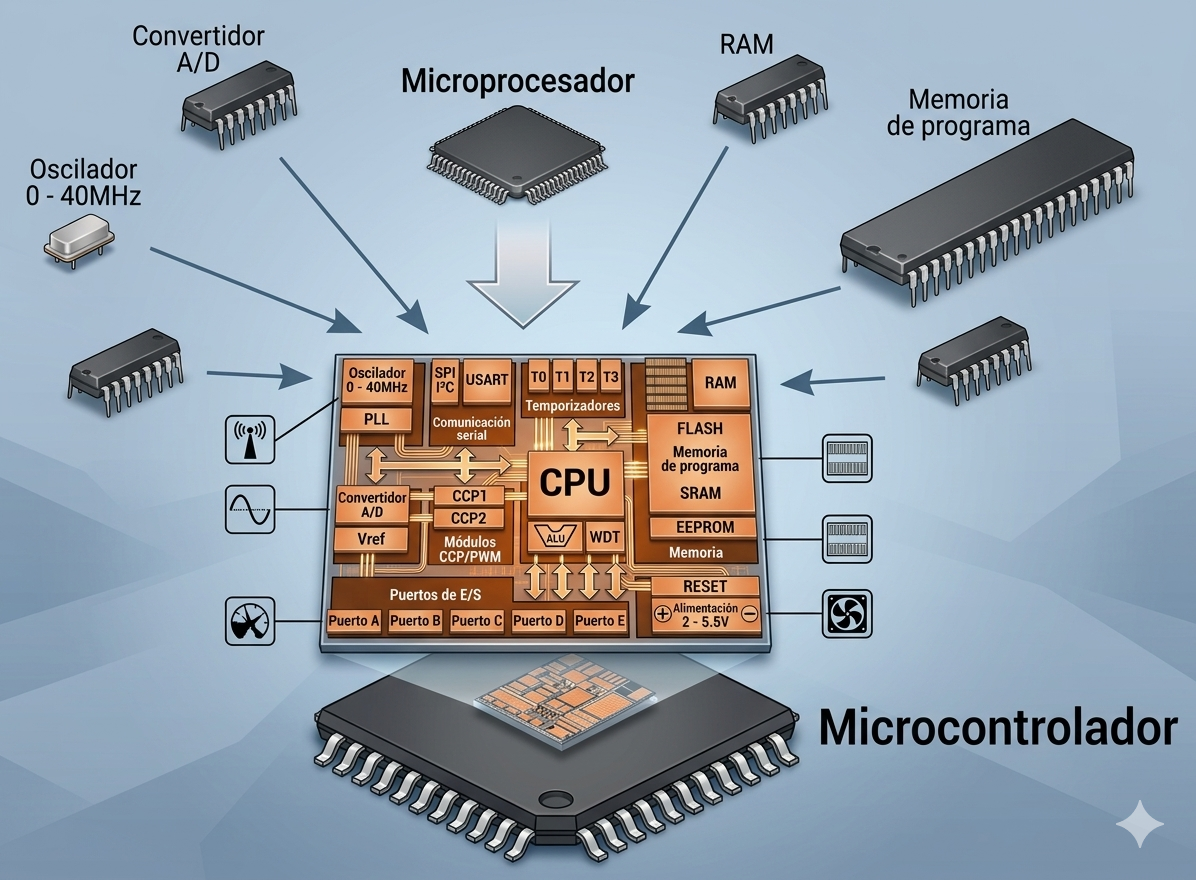
\includegraphics[width=0.75\textwidth]{Images/MICRO_E.png}
	\vspace{0.2cm}
	
	% 3. La nota de la figura según APA 7 (Con descripción técnica)
	\begin{flushleft}
		\footnotesize \textit{Nota.} Interconectividad de los componentes modulares del dispositivo, ilustrando el núcleo de procesamiento (CPU), las unidades de memoria volátil y no volátil, las líneas de los buses internos y la distribución de los periféricos de entrada y salida (I/O). Adaptado de~\citep{aprendiendoarduino2016}.
	\end{flushleft}
\end{figure}


\subsection{Programación y desarrollo de firmware}
\subsubsection{Lenguajes y paradigmas de programación}
El desarrollo de firmware para microcontroladores se realiza principalmente en lenguajes de bajo nivel pero de alto rendimiento, destacando el uso de \textit{C} y, en menor medida, \textit{C++}. Estos lenguajes permiten un control fino sobre el hardware, manejo directo de registros y periféricos, y optimización de memoria y tiempo de ejecución, aspectos críticos en sistemas embebidos de recursos limitados \citep{EmbebidosUruguay}.

En secciones críticas, como manejo de interrupciones o rutinas de tiempo real extremadamente acotado, se emplea también \textit{ensamblador} para reducir la latencia y aprovechar al máximo las características del núcleo. Además, se utilizan paradigmas de programación orientados a eventos y a tareas, mediante el uso de rutinas de servicio de interrupción (ISR), bucles principales con polling y, cuando se emplea un RTOS, ejecución de tareas concurrentes con prioridades bien definidas .

\subsubsection{Software bare‑metal y RTOS}
El \textit{bare‑metal programming} se refiere al desarrollo de firmware sin sistema operativo, donde el programador gestiona directamente el hardware, los registros y el flujo de ejecución. Este enfoque minimiza el uso de memoria y la latencia de respuesta, resultando adecuado para sistemas relativamente simples o de máxima crítica en tiempo real, como ciertas ECUs de sensado y control básico \citep{EmbebidosUruguay}.

Cuando la complejidad del sistema crece (múltiples tareas, comunicación asincrónica, gestión de recursos compartidos), se recurre a \textit{sistemas operativos en tiempo real} (RTOS) como FreeRTOS, que permiten ejecutar tareas concurrentes, gestionar colas de mensajes, semáforos y prioridades de forma determinista. Los RTOS son ampliamente utilizados en ECUs automotrices donde se requiere coordinar diversas funcionalidades (lectura de sensores, control de actuadores, comunicación CAN) con tiempos de respuesta garantizados \citep{AutomotiveEmbeddedHandbook}.

\subsubsection{Herramientas de desarrollo y depuración}
El desarrollo de firmware se apoya en una cadena de herramientas conocida como \textit{toolchain}, compuesta por compiladores (por ejemplo, GCC para ARM o herramientas del fabricante), ensambladores, enlazadores y librerías de bajo nivel. Estas herramientas transforman el código fuente en un binario que se graba en la memoria del microcontrolador y se ejecuta en el sistema objetivo .

La depuración se realiza mediante interfaces como JTAG o SWD, que permiten detener la ejecución, inspeccionar variables, modificar el flujo de control y monitorear señales de control en tiempo real. Entornos de desarrollo integrados (IDE) y simuladores ayudan a realizar pruebas tempranas y a validar algoritmos sin necesidad de hardware físico, aumentando la productividad y reduciendo errores en el diseño de firmware \citep{EmbebidosUruguay}.

\subsubsection{Pruebas y validación de firmware}
La validación de firmware incluye pruebas unitarias, pruebas de integración y, en sistemas críticos, pruebas en configuración hardware in the loop (HIL), donde la ECU se conecta a un simulador de vehículo que replica el comportamiento de sensores y actuadores. Estas pruebas permiten verificar el cumplimiento de requisitos de funcionalidad, seguridad y tiempo real antes de la puesta en marcha en el vehículo real \citep{AutomotiveEmbeddedHandbook}.

Además, se emplean técnicas de análisis estático de código, inspección de cubrimiento de pruebas y auditorías de seguridad funcional para detectar errores tempranos y asegurar que el firmware cumpla con normas de calidad y estándares de la industria automotriz.

\subsection{Comunicación y redes embebidas en automoción}
\subsubsection{CAN / CAN‑FD}
El bus \textit{CAN} (Controller Area Network), definido por la norma ISO 11898, es el estándar de comunicación más extendido en vehículos modernos. Permite interconectar múltiples unidades de control electrónico (ECU) mediante un par trenzado y protocolo de comunicación de mensajes orientado a datos, con alta inmunidad al ruido y mecanismos de arbitraje basados en la prioridad de la identificación de mensaje \citep{AutomotiveEmbeddedHandbook}.

CAN‑FD (CAN with Flexible Data Rate) es una evolución que mantiene compatibilidad con CAN clásico, pero permite velocidades de línea y tamaños de payload mayores, lo que mejora el ancho de banda disponible para datos de diagnóstico, sensores de alto volumen y sistemas ADAS. En sistemas embebidos automotrices, el uso de CAN/CAN‑FD es fundamental para la coordinación de ECUs de motor, transmisión, chasis y seguridad de forma robusta y determinista.

\subsubsection{LIN, FlexRay y Automotive Ethernet}
El bus \textit{LIN} (Local Interconnect Network) se utiliza para redes de bajo costo y baja velocidad, orientadas a subsistemas de confort y body electronics, como ventanas, cerraduras, sensores de puerta y luces interiores. LIN funciona sobre un solo cable y emplea una arquitectura maestro‑esclavo, lo que lo hace adecuado para aplicaciones no críticas en tiempo real pero sensibles al costo \citep{ AutomotiveEmbeddedHandbook}.

\textit{FlexRay} ofrece un bus de alta velocidad y alta fiabilidad, orientado a sistemas de tiempo real estricto como control de estabilidad, suspensión activa y algunas arquitecturas de seguridad. Proporciona latencias predecibles y tolerancia a fallos, pero con un costo de hardware y desarrollo más elevado respecto a CAN. En paralelo, \textit{Automotive Ethernet} aparece como solución para sistemas de alto ancho de banda, como infoentretenimiento, telemetría avanzada y comunicaciones entre dominios mediante redes IP dentro del vehículo.

\subsubsection{Protocolos de diagnóstico (OBD‑II, UDS)}
La normativa internacional de diagnósticos vehiculares se basa principalmente en el \textit{OBD‑II} (On‑Board Diagnostics II), que define formatos de conectores, mensajes básicos y códigos de fallo genéricos accesibles mediante lectores comerciales. Este protocolo permite la lectura remota de códigos DTC, el monitoreo de parámetros de funcionamiento y el borrado de fallos, facilitando el mantenimiento y la verificación emisiones \citep{ AutomotiveEmbeddedHandbook}.

Por encima de la capa física y de transporte se encuentra el protocolo \textit{UDS} (Unified Diagnostic Services, ISO 14229), que define servicios estandarizados como lectura y escritura de datos de diagnóstico, arranque de rutinas, acceso a memoria y reprogramación de firmware vía CAN (ISO 15765). 

\subsection{Requisitos eléctricos y ambientales}
\subsubsection{Rangos de tensión y transientes}

Los microcontroladores empleados en entornos automotrices deben operar de forma confiable dentro de un sistema eléctrico cuya tensión nominal es de 12\,V en vehículos de combustión interna convencionales, 24\,V en vehículos comerciales y camiones pesados, y 48\,V en arquitecturas de red de a bordo híbridas de tipo \textit{mild-hybrid} \citep{Zimmermann2014}.

La norma \textbf{ISO~16750-2} \citep{ISO16750} establece los perfiles de tensión que todo componente electrónico automotriz debe tolerar, clasificándolos en condiciones de operación normal, condiciones límite y eventos transitorios. En condiciones normales, la tensión de batería de un sistema de 12\,V oscila entre 9\,V y 16\,V durante la operación del alternador.

Los principales fenómenos transitorios reconocidos por \textbf{ISO~7637-2} 
\citep{ISO7637} e \textbf{ISO~16750-2} se describen a continuación:

\begin{itemize}
	\item \textbf{Pulso 1 — Load Dump:} Ocurre cuando la batería se desconecta 
	abruptamente mientras el alternador está en plena carga. Genera pulsos de 
	tensión que pueden superar los $+100$\,V con una duración de hasta 400\,ms. 
	Es el transitorio de mayor energía y requiere supresores de tensión tipo TVS 
	(\textit{Transient Voltage Suppressor}) o varistores de óxido metálico (MOV) 
	en la etapa de entrada de alimentación \citep{Tarter1991}.
	
	\item \textbf{Pulso 2a/2b — Interrupción inductiva:} Producido por la apertura 
	de cargas inductivas (relés, solenoides). Genera pulsos negativos de hasta 
	$-100$\,V y pulsos positivos de corta duración en el bus.
	
	\item \textbf{Pulso 3a/3b — Switching transients:} Originados por la 
	conmutación de cargas en el mismo bus. Presentan amplitudes de $\pm100$\,V 
	con duraciones del orden de los microsegundos y alta repetitividad.
	
	\item \textbf{Pulso 4 — Arranque del motor:} Durante el encendido, el motor 
	de arranque produce una caída de tensión que puede llevar el bus de 12\,V 
	hasta valores de 4--6\,V por intervalos de hasta 150\,ms. Los 
	microcontroladores deben mantener su estado operativo o ejecutar un 
	\textit{reset} controlado en este escenario \citep{Bosch2014}.
	
	\item \textbf{Pulso 5a/5b — Jump start / sobretensión de carga:} Un arranque 
	con cables de puente puede elevar la tensión hasta 24\,V en un sistema de 
	12\,V. Los reguladores de tensión de la ECU deben absorber esta condición 
	sin degradarse.
\end{itemize}

La Figura~\ref{fig:transitorios_automotriz} ilustra de forma esquemática la 
morfología temporal de los pulsos más representativos sobre un bus de 12\,V.

\begin{figure}[h]
	\centering
	
	% 1. El caption automático estilo APA 7 (Título descriptivo arriba)
	\caption{Perfiles morfológicos de los principales transitorios de tensión en un sistema eléctrico automotriz de 12\,V}
	\label{fig:transitorios_automotriz}
	\vspace{0.3cm}
	
	% 2. La imagen ajustada proporcionalmente para mantener simetría visual
	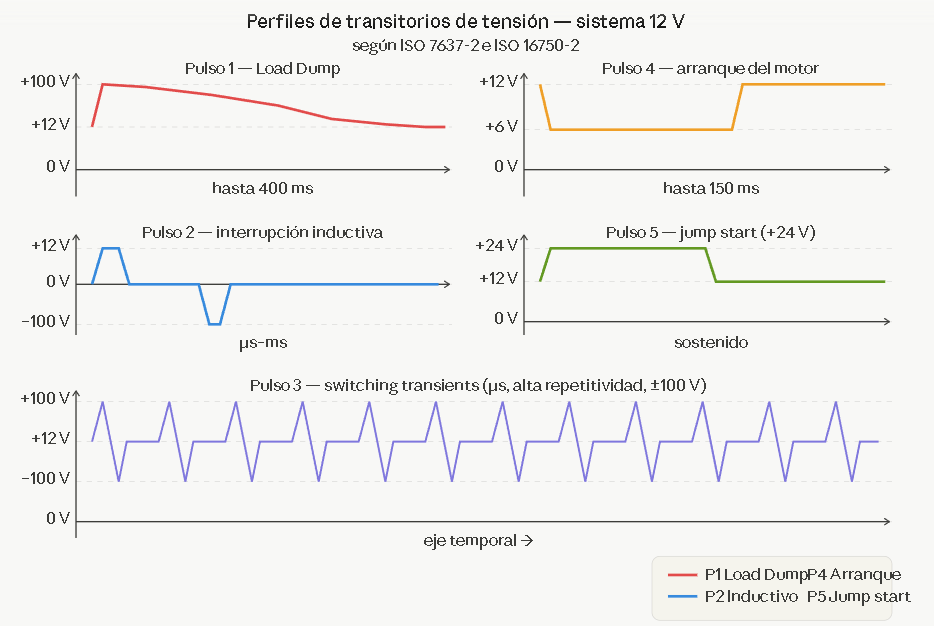
\includegraphics[width=0.95\textwidth]{Images/transitorios_automotriz.png}
	\vspace{0.2cm}
	
	% 3. La nota de la figura según APA 7 (Con la descripción y normas técnicas completas)
	\begin{flushleft}
		\footnotesize \textit{Nota.} Comportamiento temporal y formas de onda de los pulsos de voltaje críticos conforme a las normativas ISO~7637-2 e ISO~16750-2. Los pulsos 1 y 5 representan las condiciones de mayor descarga de energía (como el fenómeno de \textit{Load Dump}), mientras que el pulso 3 detalla las ráfagas de alta frecuencia provocadas por conmutaciones de relés y acoplamientos capacitivos. Elaboración propia.
	\end{flushleft}
\end{figure}

Para garantizar la integridad de las ECU frente a estos eventos, los diseñadores 
recurren a una cadena de protección en la etapa de entrada de alimentación que 
combina varios dispositivos \citep{Bosch2014}:

\begin{enumerate}
	\item \textbf{Fusible o PTC:} Primera barrera contra sobrecorriente sostenida.
	
	\item \textbf{MOV / TVS bidireccional:} Absorbe la energía del Load Dump y 
	los pulsos positivos de alta tensión. Los diodos TVS (p.\,ej., serie SMBJ) 
	ofrecen tiempos de respuesta del orden de los picosegundos.
	
	\item \textbf{Inductor de modo común y condensador de desacoplo:} Filtra los 
	transitorios de alta frecuencia (pulso~3) y desacopla el bus de la 
	electrónica interna.
	
	\item \textbf{Regulador de tensión (LDO o SMPS):} Provee la tensión 
	estabilizada de 5\,V o 3{,}3\,V al MCU, con rechazo de rizado (PSRR) y 
	protección de subvoltaje (\textit{undervoltage lockout}, UVLO) para gestionar 
	correctamente la caída producida durante el arranque (pulso~4).
	
	\item \textbf{Supervisor de tensión:} Circuito dedicado (p.\,ej., TPS3840) 
	que monitoriza continuamente la alimentación y genera un \textit{reset} 
	controlado ante condiciones fuera de rango, garantizando la integridad del 
	firmware almacenado en memoria no volátil.
\end{enumerate}

Los microcontroladores automotrices modernos, como el Renesas RH850 o el 
NXP~S32K3, incorporan internamente circuitos de UVLO y detectores de 
\textit{brown-out} conformes con los requisitos de ISO~16750-2, reduciendo la 
cantidad de componentes externos necesarios en el diseño de la ECU 
\citep{Renesas2021, NXP2022}.


%%%─────────────────────────────────────────────────────────────
\subsection{Aplicaciones en la industria automotriz}

Los microcontroladores (MCU) constituyen el núcleo computacional de las
unidades de control electrónico (\textit{Electronic Control Unit}, ECU) que
gobiernan la práctica totalidad de los subsistemas de un vehículo moderno.
Según estimaciones de la industria, un automóvil de gama media-alta incorpora
entre 70 y 100 ECUs independientes, cifra que en vehículos premium o eléctricos
puede superar las 150 unidades \citep{Bosch2014}. Estas ECUs se agrupan
funcionalmente en dominios que comparten buses de comunicación, requisitos de
integridad y restricciones de tiempo real, tal como se ilustra en la
Figura~\ref{fig:dominios_ecu}.

\begin{figure}[h]
	\centering
	
	% 1. El caption automático estilo APA 7 (Título descriptivo conciso arriba)
	\caption{Arquitectura y distribución de dominios de ECUs en un vehículo moderno}
	\label{fig:dominios_ecu}
	\vspace{0.3cm}
	
	% 2. La imagen ajustada proporcionalmente para mantener simetría visual
	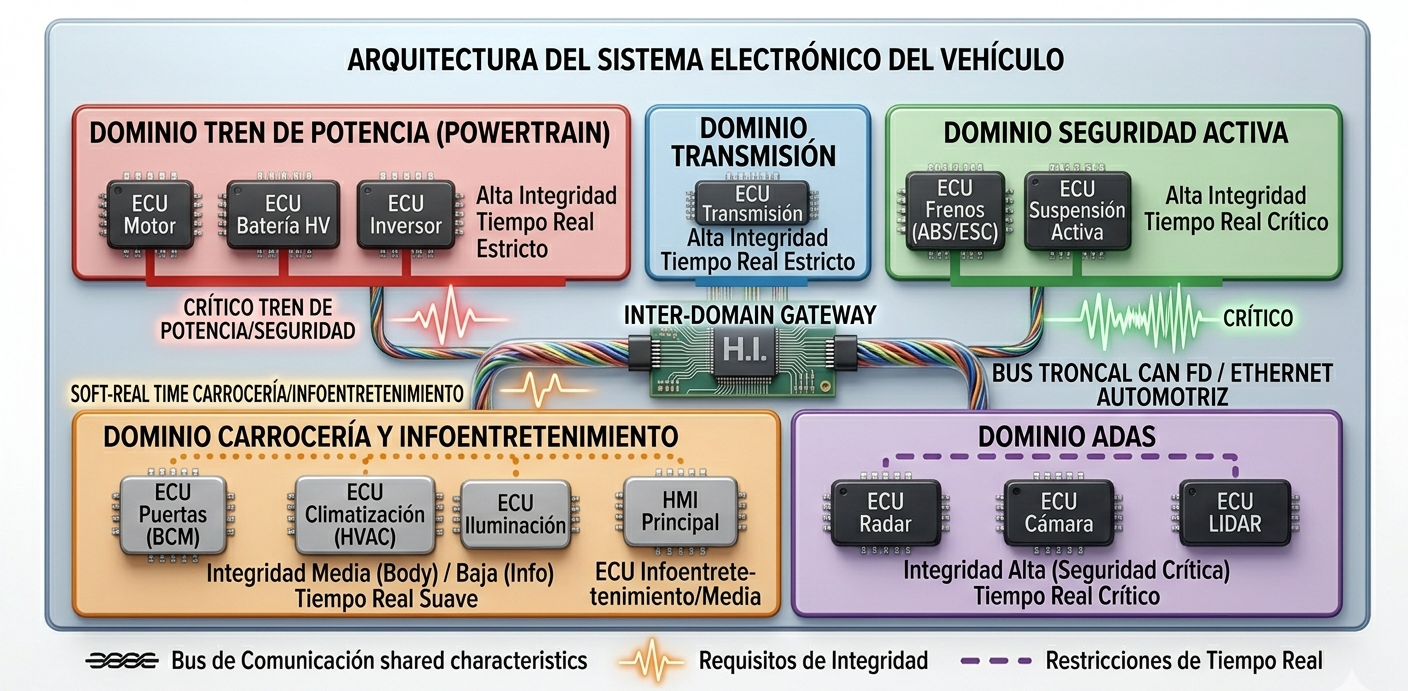
\includegraphics[width=0.95\textwidth]{Images/dominios_ecu.png}
	\vspace{0.2cm}
	
	% 3. La nota de la figura según APA 7 (Con la descripción técnica detallada)
	\begin{flushleft}
		\footnotesize \textit{Nota.} Organización funcional del sistema electrónico del vehículo dividida en cinco dominios principales: \textit{powertrain}, transmisión, seguridad activa, \textit{body}/infoentretenimiento y sistemas avanzados de asistencia al conductor (ADAS). Se ilustra la interconectividad y el flujo de datos masivo a través de un bus troncal central basado en las tecnologías CAN\,FD y Ethernet automotriz. Elaboración propia.
	\end{flushleft}
\end{figure}

%%%─────────────────────────────────────────────────────────────
\subsection{ECUs de powertrain}

El dominio de \textit{powertrain} agrupa las ECUs responsables de la gestión
energética del tren de potencia, siendo la más relevante la unidad de control
del motor (\textit{Engine Management System}, EMS o ECM). Su función principal
consiste en optimizar los procesos de dosificación de combustible, encendido y
control de emisiones, garantizando simultáneamente el rendimiento dinámico
exigido por el conductor y el cumplimiento de las normativas de emisiones
EURO\,6d y EPA Tier\,3 \citep{Reif2015}.

\subsubsection{Funciones principales de la ECM}

La ECM adquiere señales de un conjunto de sensores —cigüeñal, árbol de levas,
masa de aire (MAF), presión absoluta en colector (MAP), sonda lambda de banda
ancha, temperatura de refrigerante y presión de combustible— y ejecuta, en
tiempo real, los algoritmos de:

\begin{itemize}
	\item \textbf{Cálculo de tiempo de inyección (\textit{injection pulse width},
		IPW):} basado en modelos de carga volumétrica y correcciones adaptativas
	por desvíos lambda \citep{Bosch2014}.
	\item \textbf{Avance de encendido:} optimizado ciclo a ciclo mediante el
	detector de detonación (\textit{knock sensor}); en motores modernos
	con encendido por compresión (HCCI), el control se realiza
	por temperatura en cámara \citep{Heywood2018}.
	\item \textbf{Gestión del par:} coordinación con la TCU y con el sistema
	ESP para garantizar transferencia de par coherente en maniobras de
	cambio o corrección de estabilidad.
	\item \textbf{Control de emisiones:} regeneración del filtro de partículas
	(DPF), dosificación de AdBlue para reducción catalítica selectiva (SCR)
	y monitorización del sistema OBD-II conforme a ISO~15031 \citep{sae_j1979_2014}.
\end{itemize}

\subsubsection{Requerimientos computacionales}

La ECM opera con ciclos de control de hasta 1\,ms para las tareas de alta
prioridad (inyección, encendido) y ciclos de 10--100\,ms para las tareas de
diagnóstico y adaptación. Esto impone el uso de MCUs de 32\,bits con núcleos
duales en configuración \textit{lockstep} —como el Infineon AURIX TC3xx o el
NXP S32K3— capaces de ejecutar entre 200 y 800\,DMIPS con memorias Flash de
hasta 16\,MB y RAM de hasta 6\,MB \citep{Infineon2022, NXP2022} ver Tabla \ref{tab:mcu_ecm}.

\begin{table}[h]
	\centering
	% Título separado bajo norma estricta APA 7
	\captionsetup{labelformat=simple, labelsep=newline, textfont=it, labelfont=bf}
	\caption{Parámetros típicos de microcontroladores utilizados en módulos de control de motor de producción}
	\label{tab:mcu_ecm}
	
	% Ajuste de espaciado vertical de filas para una lectura cómoda
	\renewcommand{\arraystretch}{1.25}
	
	% Usamos tabularx con alineación centrada para las columnas cuantitativas
	\begin{tabularx}{\linewidth}{X c c c c c}
		\toprule % Línea superior APA 7
		\rowcolor[rgb]{0.851, 0.851, 0.851}
		\textbf{Familia} & \textbf{Núcleos} & \textbf{Frec. (MHz)} & \textbf{Flash (MB)} & \textbf{RAM (KB)} & \textbf{ASIL} \\
		\midrule % Línea divisoria de encabezado APA 7
		AURIX TC39x & 6 $\times$ TriCore & 300 & 16 & 6\,272 & D \\
		\addlinespace
		S32K396 & 4 $\times$ CM7 & 320 & 16 & 4\,096 & D \\
		\addlinespace
		RH850/U2A & 8 $\times$ G4MH & 400 & 16 & 7\,680 & D \\
		\addlinespace
		SPC58xEx & 4 $\times$ e200z7 & 200 & 8 & 1\,536 & D \\
		\bottomrule % Línea inferior de cierre APA 7
	\end{tabularx}
	\vspace{0.2cm}
	
	\begin{flushleft}
		\footnotesize \textit{Nota.} Criterios de rendimiento, almacenamiento y niveles de integridad de seguridad de la arquitectura automotriz (ASIL) en semiconductores integrados para la gestión del \textit{powertrain}. Elaboración propia.
	\end{flushleft}
\end{table}

La arquitectura \textit{lockstep} duplica la ejecución en dos núcleos idénticos
comparando los resultados en cada ciclo de reloj; cualquier discrepancia activa
un manejador de fallo seguro, lo que constituye un requisito indispensable
para alcanzar el nivel ASIL-D según ISO~26262 \citep{ISO16750}.

%%%─────────────────────────────────────────────────────────────
%\subsection{Control de transmisión (TCU)}
%
%La unidad de control de transmisión (\textit{Transmission Control Unit}, TCU)
%gestiona la lógica de cambio de marchas, la presión hidráulica de los embragues
%y la coordinación de par entre el motor y la caja de cambios \citep{Naunheimer2011}.
%En transmisiones automáticas de convertidor de par (AT), de doble embrague (DCT)
%y de variación continua (CVT), la TCU es la pieza central que determina el
%confort de cambio, la eficiencia energética y la protección mecánica del conjunto.
%
%\subsubsection{Estrategias de control}
%
%Las TCUs modernas implementan tres capas de control:
%
%\begin{enumerate}
%	\item \textbf{Capa de estrategia:} decide el punto de cambio óptimo a partir
%	de mapas multidimensionales que relacionan velocidad del vehículo, posición
%	del acelerador, pendiente de la calzada (estimada por el acelerómetro del
%	ESP) y modo de conducción seleccionado (Sport, Eco, Manual).
%	\item \textbf{Capa de control hidráulico:} regula solenoides de presión y
%	flujo con lazos PID de alta velocidad (ciclos de 1--5\,ms) para garantizar
%	el llenado y vaciado de los embragues dentro de las ventanas de tiempo de
%	cambio establecidas ($<$600\,ms en AT convencional,
%	$<$200\,ms en DCT) \citep{Naunheimer2011}.
%	\item \textbf{Capa de coordinación:} se comunica con la ECM vía CAN para
%	solicitar reducciones de par durante el cambio y evitar el impacto de
%	tracción (\textit{shift shock}).
%\end{enumerate}
%
%\subsubsection{Comunicación y diagnóstico}
%
%La TCU opera en el bus CAN\,HS a 500\,kbit/s e intercambia tramas con la ECM,
%el módulo ABS/ESP y la pantalla de instrumentos. A través del protocolo
%UDS (ISO~14229) expone parámetros de diagnóstico (temperatura de aceite,
%presión de embrague, número de cambios acumulados) accesibles con herramientas
%OBD-II de taller \citep{ISO14229} Algunas comparatuvas se presentan en la Tabla \ref{tab:tipos_tcu}.
%
%\begin{table}[h]
%	\centering
%	% Título separado bajo norma estricta APA 7
%	\captionsetup{labelformat=simple, labelsep=newline, textfont=it, labelfont=bf}
%	\caption{Comparativa de tipos de transmisión automática y requisitos de la unidad de control de transmisión}
%	\label{tab:tipos_tcu}
%	
%	% Ajuste de espaciado vertical de filas para mantener consistencia visual
%	\renewcommand{\arraystretch}{1.25}
%	
%	% Usamos tabularx con alineación centrada para las columnas de datos de ingeniería
%	\begin{tabularx}{\linewidth}{X c c c c}
%		\toprule % Línea superior APA 7
%		\rowcolor[rgb]{0.851, 0.851, 0.851}
%		\textbf{Tipo} & \textbf{Ciclo ctrl.} & \textbf{Solenoides} & \textbf{Bus CAN} & \textbf{ASIL} \\
%		\midrule % Línea divisoria de encabezado APA 7
%		AT conv. (6--10 vel.) & 5\,ms & 6--10 & HS 500 kbit/s & B \\
%		\addlinespace
%		DCT (7 vel.) & 1\,ms & 12--16 & HS 500 kbit/s & C \\
%		\addlinespace
%		CVT & 2\,ms & 4--6 & HS 500 kbit/s & B \\
%		\addlinespace
%		Híbrido P2 (DCT + motor) & 1\,ms & 16+ & CAN FD 2 Mbit/s & C \\
%		\bottomrule % Línea inferior de cierre APA 7
%	\end{tabularx}
%	\vspace{0.2cm}
%	
%	\begin{flushleft}
%		\footnotesize \textit{Nota.} Criterios de diseño temporal, demanda de actuadores hidráulicos, velocidad del bus de datos y requerimientos de seguridad funcional (ASIL) según la arquitectura de la transmisión. Elaboración propia.
%	\end{flushleft}
%\end{table}
%
%%%%─────────────────────────────────────────────────────────────
%\subsection{Sistemas de seguridad}
%
%Los sistemas de seguridad activa constituyen el dominio de mayor criticidad
%funcional del vehículo. Sus ECUs deben alcanzar el nivel ASIL-D —el más
%elevado de la norma ISO~26262— y garantizar la ejecución correcta de sus
%funciones incluso ante fallos de hardware o software \citep{ISO16750}.
%Este dominio comprende principalmente: el módulo de control de frenos
%(ABS/ESP/TCS), el actuador de dirección asistida eléctrica (EPS) y la unidad
%de control del airbag (ACU).
%
%\subsubsection{ABS / ESP / TCS}
%
%El sistema antibloqueo de frenos (ABS) y el programa electrónico de
%estabilidad (ESP) comparten una ECU que adquiere señales de velocidad en
%cada rueda (sensores de efecto Hall ABS), aceleración lateral e
%inercial (IMU de 6 ejes) y presión en el circuito de frenos. El algoritmo
%ESP detecta la divergencia entre la trayectoria deseada (calculada a partir
%del ángulo de volante y la velocidad del vehículo) y la real (medida con el
%giróscopo de guiñada), aplicando frenadas selectivas en las ruedas individua\-les
%con una resolución de par de 1\,Nm y tiempos de respuesta inferiores a
%20\,ms \citep{Bosch2014}.
%
%La ECU del ESP opera típicamente con un MCU de arquitectura \textit{lockstep}
%a 160--200\,MHz, conectado a dos módulos de accionamiento hidráulico mediante
%un bus privado de alta velocidad (FlexRay a 10\,Mbit/s o CAN\,FD a 5\,Mbit/s)
%para minimizar la latencia de actuación \citep{FlexRay2010}.
%
%\subsubsection{Unidad de control del airbag (ACU)}
%
%La ACU monitoriza de forma continua (período de muestreo de 1\,ms)
%los acelerómetros de impacto periféricos y el sensor central de desaceleración.
%Un algoritmo de fusión de señales evalúa en tiempo real si la severidad del
%impacto supera el umbral de disparo, tomando la decisión de activar los
%pirotécnicos de los airbags en menos de 15\,ms desde el inicio del impacto,
%tiempo durante el cual el vehículo apenas ha deformado los primeros 30\,mm
%de la zona de absorción \citep{Bastian2016}.
%
%La ACU implementa redundancia en la fuente de alimentación: un
%\textit{energy reserve capacitor} almacena suficiente energía para disparar
%todos los airbags incluso si la batería queda desconectada en el impacto,
%cumpliendo con el requisito ASIL-D de disponibilidad de misión
%(\textit{mission time}) de al menos 150\,ms.
%
%\subsubsection{Dirección asistida eléctrica (EPS)}
%
%La ECU de EPS controla un motor BLDC de 200--1\,000\,W acoplado a la columna
%de dirección. El lazo de control de corriente opera a 20\,kHz, mientras el
%lazo de par asistido opera a 1\,kHz. La función de asistencia se mapea en
%función de la velocidad del vehículo (a baja velocidad se asiste más para
%facilitar maniobras, a alta velocidad menos para mejorar la retroalimentación
%al conductor) \citep{Reif2015}. En sistemas de dirección autónoma de nivel 3+,
%la EPS recibe trayectorias objetivo desde el dominio ADAS y actúa como
%actuador de seguimiento con ASIL-D ver Tabla \ref{tab:ecu_seguridad}.
%
%\begin{table}[h]
%	\centering
%	% Título separado bajo norma estricta APA 7
%	\captionsetup{labelformat=simple, labelsep=newline, textfont=it, labelfont=bf}
%	\caption{ECUs de seguridad activa: función, bus y nivel ASIL requerido}
%	\label{tab:ecu_seguridad}
%	
%	% Ajuste de espaciado vertical de las filas
%	\renewcommand{\arraystretch}{1.25}
%	
%	% Usamos tabularx para garantizar la adaptación a los márgenes del documento
%	\begin{tabularx}{\linewidth}{l X c c c}
%		\toprule % Línea superior APA 7
%		\rowcolor[rgb]{0.851, 0.851, 0.851}
%		\textbf{ECU} & \textbf{Función principal} & \textbf{Bus} & \textbf{Ciclo ctrl.} & \textbf{ASIL} \\
%		\midrule % Línea divisoria de encabezado APA 7
%		ABS/ESP & Estabilidad dinámica y control de tracción. & CAN FD / FlexRay & 1\,ms & D \\
%		\addlinespace
%		ACU & Gestión y disparo de \textit{airbags} (bolsas de aire). & CAN HS & 1\,ms & D \\
%		\addlinespace
%		EPS & Control y asistencia de la dirección eléctrica. & CAN FD & 0.05\,ms & D \\
%		\addlinespace
%		EPB & Freno de estacionamiento electromecánico. & LIN / CAN & 10\,ms & C \\
%		\addlinespace
%		BBW & Sistema de frenado electrónico (\textit{Brake-by-wire}). & FlexRay & 1\,ms & D \\
%		\bottomrule % Línea inferior de cierre APA 7
%	\end{tabularx}
%	\vspace{0.2cm}
%	
%	\begin{flushleft}
%		\footnotesize \textit{Nota.} Análisis de la latencia temporal y requerimientos de confiabilidad crítica en los sistemas electrónicos orientados a la mitigación de colisiones y seguridad dinámica del vehículo. Elaboración propia.
%	\end{flushleft}
%\end{table}
%
%%%%─────────────────────────────────────────────────────────────
%\subsection{Body electronics e infoentretenimiento}
%
%El dominio de \textit{body electronics} agrupa las funciones de confort,
%iluminación, control climático y acceso al vehículo, cuya criticidad funcional
%es generalmente baja (QM o ASIL-A) pero cuyo volumen es elevado: puede
%representar hasta el 40\,\% de las ECUs totales del vehículo \citep{Zimmermann2014}.
%La tendencia actual es consolidar estas funciones en módulos de zona
%(\textit{zone controllers}) que sustituyen a decenas de nodos LIN
%dispersos \citep{AUTOSAR2023}.
%
%\subsubsection{Módulo de control de carrocería (BCM)}
%
%El BCM centraliza el control de:
%
%\begin{itemize}
%	\item \textbf{Iluminación exterior e interior:} gestión PWM de LEDs de alta
%	potencia (faros matriciales, luces DRL, indicadores de posición),
%	incluyendo funciones de curvado adaptativo y encendido automático.
%	\item \textbf{Elevalunas, retrovisores y techo solar:} accionamiento de
%	motores DC con detección de obstáculos por monitorización de corriente
%	(\textit{anti-pinch}).
%	\item \textbf{Acceso y arranque sin llave (PASE):} comunicación LF/RF con
%	la llave inteligente, autenticación por criptografía AES-128 y
%	activación del relé de encendido.
%	\item \textbf{Climatización (HVAC):} regulación PID de temperatura en
%	cabina, control de velocidad del ventilador y distribución de
%	flujo de aire por compuertas servoaccionadas.
%\end{itemize}
%
%El bus LIN es el protocolo predominante en este dominio: opera a
%10.4--20\,kbit/s, es de bajo coste (bus de un solo hilo) y es adecuado
%para esclavos de baja velocidad como sensores de lluvia, motores de apertura
%y actuadores de HVAC \citep{LIN2016}. El BCM actúa como maestro LIN y
%a su vez como nodo CAN, puente entre los dos dominios.
%
%\subsubsection{Infoentretenimiento y conectividad}
%
%La unidad de infoentretenimiento (\textit{Head Unit} o IVI,
%\textit{In-Vehicle Infotainment}) es la ECU de mayor complejidad software
%del dominio. Ejecuta un sistema operativo embebido (Android Automotive OS,
%QNX Neutrino o Linux con Yocto) sobre un SoC de aplicaciones (p.\,ej.,
%Qualcomm SA8295P o Renesas R-Car H3) con CPU de 8 núcleos a 3\,GHz,
%GPU integrada, acelerador neuronal y hasta 8\,GB de RAM \citep{Qualcomm2022}.
%
%Sus funciones incluyen:
%
%\begin{itemize}
%	\item Navegación con mapas vectoriales en tiempo real (HERE, TomTom).
%	\item Conectividad inalámbrica: Wi-Fi 802.11ac, Bluetooth 5.x,
%	Apple CarPlay y Android Auto vía USB/Wi-Fi.
%	\item Transmisión de video 4K para cámaras de 360° y pantallas traseras.
%	\item \textit{Over-the-Air} (OTA): actualización del firmware del IVI
%	y de otras ECUs vía red 4G/5G, conforme a UNECE WP.29
%	R156 \citep{UNECE_R156}.
%\end{itemize}
%
%Algunas protocolomas mas usados en este dominio se presentan en la Tabla \ref{tab:protocolos_body}.
%
%\begin{table}[h]
%	\centering
%	% Título separado bajo norma estricta APA 7
%	\captionsetup{labelformat=simple, labelsep=newline, textfont=it, labelfont=bf}
%	\caption{Protocolos de comunicación predominantes en el dominio de confort e infoentretenimiento}
%	\label{tab:protocolos_body}
%	
%	% Ajuste de espaciado vertical de las filas para mantener la consistencia
%	\renewcommand{\arraystretch}{1.25}
%	
%	% Usamos tabularx para un ajuste milimétrico automático entre los márgenes
%	\begin{tabularx}{\linewidth}{l c c c X}
%		\toprule % Línea superior APA 7
%		\rowcolor[rgb]{0.851, 0.851, 0.851}
%		\textbf{Protocolo} & \textbf{Velocidad} & \textbf{Topología} & \textbf{Nodos máx.} & \textbf{Aplicación típica} \\
%		\midrule % Línea divisoria de encabezado APA 7
%		LIN 2.2A & 20 kbit/s & Bus (1 hilo) & 16 & Sensores de lluvia, espejos eléctricos y sistemas HVAC. \\
%		\addlinespace
%		CAN HS & 1 Mbit/s & Bus pasivo & 32 & Módulo de control de carrocería (BCM), \textit{gateway} e instrumentación. \\
%		\addlinespace
%		MOST150 & 150 Mbit/s & Anillo óptico & 64 & Sistemas de audio de alta fidelidad y vídeo digital. \\
%		\addlinespace
%		Ethernet & Hasta 1 Gbit/s & Estrella & --- & Infoentretenimiento (IVI), sistemas de cámaras y pasarelas OTA. \\
%		\bottomrule % Línea inferior de cierre APA 7
%	\end{tabularx}
%	\vspace{0.2cm}
%	
%	\begin{flushleft}
%		\footnotesize \textit{Nota.} Comparación de estándares de red según su tasa de transferencia de datos, distribución geométrica y aplicaciones en el entorno de confort y telemática del vehículo. Elaboración propia.
%	\end{flushleft}
%\end{table}
%
%%%%─────────────────────────────────────────────────────────────
%\subsection{ADAS y fusión de sensores}
%
%Los sistemas avanzados de asistencia al conductor (\textit{Advanced Driver
%Assistance Systems}, ADAS) representan el dominio de mayor crecimiento en laelectrónica automotriz, impulsado por la hoja de ruta de automatización SAE J3016 que define seis niveles de autonomía (L0--L5) \citep{SAE_J3016}. Las ECUs de ADAS deben procesar flujos de datos de múltiples modalidades sensoriales, fusionarlos en una representación del entorno y alimentar los algoritmos de percepción, planificación y control que gobiernan la respuesta del vehículo.
%
%\subsubsection{Modalidades sensoriales}
%
%Cada sensor tiene características de alcance, resolución y robustez ambiental
%complementarias, lo que hace indispensable la fusión de datos ver Tabla \ref{tab:sensores_adas}:
%
%\begin{table}[htbp]
%	\centering
%	% Título separado bajo norma estricta APA 7
%	\captionsetup{labelformat=simple, labelsep=newline, textfont=it, labelfont=bf}
%	\caption{Comparativa de sensores empleados en sistemas avanzados de asistencia al conductor y sus características operativas}
%	\label{tab:sensores_adas}
%	
%	% Ajuste de espaciado vertical de las filas para una lectura limpia
%	\renewcommand{\arraystretch}{1.3}
%	
%	% Asignamos anchos fijos proporcionales exactos que sumados dan 1.00\textwidth
%	\begin{tabular}{p{0.15\textwidth} p{0.10\textwidth} p{0.14\textwidth} p{0.10\textwidth} p{0.20\textwidth} p{0.11\textwidth}}
%		\toprule % Línea superior APA 7
%		\rowcolor[rgb]{0.851, 0.851, 0.851}
%		\textbf{Sensor} & \textbf{Alcance} & \textbf{Res. ang.} & \textbf{Rango vel.} & \textbf{Condic. adv.} & \textbf{Costo rel.} \\
%		\midrule % Línea divisoria de encabezado APA 7
%		Cámara mono/estéreo & 0 -- 250\,m & Alta (píxel) & Media & Bajo (lluvia, niebla) & Bajo \\
%		\addlinespace
%		Radar 77\,GHz & 0 -- 300\,m & Baja -- media & Alto & Alto & Medio \\
%		\addlinespace
%		LiDAR (ToF) & 0 -- 200\,m & Muy alta & Bajo & Medio (lluvia) & Alto \\
%		\addlinespace
%		Ultrasónico & 0 -- 5\,m & Baja & Estático & Alto & Muy bajo \\
%		\addlinespace
%		IMU (6 ejes) & --- & --- & --- & Muy alto & Bajo \\
%		\addlinespace
%		GNSS (RTK) & --- & 0.01\,m & Medio & Bajo (túneles) & Medio \\
%		\bottomrule % Línea inferior de cierre APA 7
%	\end{tabular}
%	\vspace{0.2cm}
%	
%	\begin{flushleft}
%		\footnotesize \textit{Nota.} Análisis comparativo de los rangos de operación, inmunidad a perturbaciones climáticas y costos relativos de los componentes de hardware que integran la capa de percepción del entorno vehicular. Elaboración propia.
%	\end{flushleft}
%\end{table}
%
%\subsubsection{Arquitectura de fusión de sensores}
%
%La fusión de sensores se implementa en tres capas \citep{Thrun2005}:
%
%\begin{enumerate}
%	\item \textbf{Fusión a nivel de dato (\textit{early fusion}):} combinación
%	de nubes de puntos LiDAR con imágenes de cámara en el espacio de
%	características antes de la detección de objetos. Requiere calibración
%	extrínseca precisa entre sensores.
%	\item \textbf{Fusión a nivel de objeto (\textit{mid fusion}):} cada sensor
%	genera su propia lista de objetos detectados (posición, velocidad,
%	clasificación) y un filtro de Kalman extendido (EKF) o un filtro de
%	partículas los integra en una lista de objetos fusionados
%	(\textit{object list}) con covarianza de incertidumbre \citep{Thrun2005}.
%	\item \textbf{Fusión a nivel de decisión (\textit{late fusion}):} cada
%	subsistema genera una acción recomendada y un árbitro de decisión
%	selecciona la acción más conservadora (p.\,ej., intervención de frenado
%	de emergencia).
%\end{enumerate}
%
%\subsubsection{ECUs de dominio y SoCs de ADAS}
%
%El procesamiento de ADAS exige plataformas de alto rendimiento (\textit{High
%	Performance Computing}, HPC). Los SoCs de ADAS combinan en un único chip:
%CPUs de propósito general para planificación, aceleradores de visión
%(\textit{Deep Neural Network}, DNN) para inferencia de redes convolucionales
%(YOLO, PointPillars, BEVFusion) y núcleos de seguridad funcional en
%\textit{lockstep} para las tareas de actuación ASIL-D \citep{Mobileye2021}.
%
%En la Tabla \ref{tab:soc_adas} se muestra las capacidades de SoCs en ADAS.
%
%\begin{table}[h]
%	\centering
%	% Título separado bajo norma estricta APA 7
%	\captionsetup{labelformat=simple, labelsep=newline, textfont=it, labelfont=bf}
%	\caption{SoCs de ADAS de producción masiva y sus capacidades de procesamiento computacional}
%	\label{tab:soc_adas}
%	
%	% Ajuste de espaciado vertical de las filas para consistencia visual
%	\renewcommand{\arraystretch}{1.25}
%	
%	% Usamos tabularx para garantizar la adaptación exacta a los márgenes
%	\begin{tabularx}{\linewidth}{X c c c c}
%		\toprule % Línea superior APA 7
%		\rowcolor[rgb]{0.851, 0.851, 0.851}
%		\textbf{SoC} & \textbf{Fabricante} & \textbf{TOPS (DNN)} & \textbf{Nivel SAE objetivo} & \textbf{ASIL} \\
%		\midrule % Línea divisoria de encabezado APA 7
%		EyeQ6H & Mobileye & 176 & L2+ & D \\
%		\addlinespace
%		TDA4VM & TI & 8 & L2 & D \\
%		\addlinespace
%		Xavier (AGX) & NVIDIA & 30 & L3 & B \\
%		\addlinespace
%		Orin (AGX) & NVIDIA & 254 & L4 & D \\
%		\addlinespace
%		Snapdragon Ride & Qualcomm & 700+ & L4+ & D \\
%		\bottomrule % Línea inferior de cierre APA 7
%	\end{tabularx}
%	\vspace{0.2cm}
%	
%	\begin{flushleft}
%		\footnotesize \textit{Nota.} Comparación de la capacidad de cómputo en Tera Operaciones Por Segundo (TOPS) destinadas al procesamiento de redes neuronales profundas (DNN) y su clasificación según los niveles de automatización de la SAE. Elaboración propia.
%	\end{flushleft}
%\end{table}
%
%La comunicación entre los sensores y la ECU de ADAS utiliza Ethernet automotriz 1000BASE-T1 o 100BASE-T1 (IEEE~802.3bw/bp), que permite
%transferir flujos de video comprimidos (H.265) y nubes de puntos LiDAR
%con latencias inferiores a 1\,ms, empleando el protocolo de transporte
%SOME/IP o DDS sobre una pila de red conforme a AUTOSAR Adaptive Platform
%\citep{AUTOSAR2023, SOME_IP}.
%
%La integridad funcional del dominio ADAS no se limita a ISO~26262; la
%norma ISO~21448 (SOTIF, \textit{Safety Of The Intended Functionality})
%\citep{ISO21448} aborda los fallos causados no por averías de hardware sino
%por limitaciones del sistema en condiciones no previstas durante el diseño
%(p.\,ej., condiciones de iluminación extrema que degradan la percepción
%de la cámara).

% ============================================================
\subsection{Ejemplos prácticos y casos de estudio}
% ============================================================

La literatura reporta múltiples implementaciones de sistemas
embebidos para la adquisición de datos vehiculares mediante el
protocolo OBD-II sobre bus CAN.  Estos casos de estudio
constituyen antecedentes directos del presente proyecto.

% -----------------------------------------------------------
\subsection{Medidor de consumo de combustible con microcontrolador}
% -----------------------------------------------------------

Uno de los enfoques más consolidados para estimar el consumo
de combustible en tiempo real utiliza los parámetros PID
estándar del protocolo SAE~J1979 disponibles a través del
conector OBD-II.  \citet{Rimpas2020} seleccionaron variables
como el flujo másico de aire (MAF), el sensor de lambda
($\lambda$), la temperatura del refrigerante (ECT) y la
velocidad del vehículo (VSS) para estimar el consumo
volumétrico instantáneo.  La fórmula fundamental empleada es:

\begin{equation}
	\dot{m}_{\text{fuel}} =
	\frac{\dot{m}_{\text{air}}}{\lambda \cdot \text{AFR}_{\text{stoich}}}
	\label{eq:fuel_mass}
\end{equation}

\noindent donde $\dot{m}_{\text{air}}$ es el flujo másico de
aire en g/s proporcionado por el sensor MAF y
$\text{AFR}_{\text{stoich}} = 14.7$ para gasolina.  La
conversión volumétrica se obtiene dividiendo la masa de
combustible entre su densidad energética
($\rho \approx 770$~g/l):

\begin{equation}
	\dot{V}_{\text{fuel}} =
	\frac{\dot{m}_{\text{fuel}}}{\rho_{\text{fuel}}}
	\label{eq:fuel_volume}
\end{equation}

Para expresar el consumo en \mbox{L/100~km} se divide la
distancia recorrida entre los litros consumidos y se invierte
la relación.  Cuando el sensor MAF no está disponible, como
ocurre en algunos vehículos Chrysler y Honda, se emplea el
modelo \textit{Speed-Density} basado en la presión absoluta
del múltiple de admisión (MAP) y la ley del gas ideal
\citep{HEMData2021}.

\citet{Ling2021} propusieron un sistema de adquisición de
datos embebido orientado a flotas de transporte público,
combinando un módulo OBD-II sobre CAN con un receptor GPS para
correlacionar el estilo de conducción con el consumo.  Sus
resultados mostraron que en condiciones urbanas la
incertidumbre de medición del consumo puede alcanzar el 7~\%.
\citet{FuelConsumptionSVM2020} validaron la estimación de
consumo usando PIDs de RPM y posición del acelerador (TPS)
sobre tres vehículos de distintas marcas (Ford~Fusion~2017,
Mercedes-Benz~E280~2006 y Toyota~Camry~2016), logrando buenos
ajustes con modelos de máquina de soporte vectorial (SVM).

La Tabla~\ref{tab:pids_consumo} resume los PIDs del estándar
SAE~J1979 más empleados en proyectos de medición de consumo:

\begin{table}[h]
	\centering
	% Título separado bajo norma estricta APA 7
	\captionsetup{labelformat=simple, labelsep=newline, textfont=it, labelfont=bf}
	\caption{PIDs OBD-II relevantes para el cálculo de consumo de combustible}
	\label{tab:pids_consumo}
	
	% Ajuste de espaciado vertical base de las filas
	\renewcommand{\arraystretch}{1.3}
	
	% Forzamos a la tabla completa a ajustarse de forma compacta al ancho de página
	\resizebox{\textwidth}{!}{%
		\begin{tabular}{c l c p{8.5cm}}
			\toprule % Línea superior APA 7
			\rowcolor[rgb]{0.851, 0.851, 0.851}
			\textbf{PID (hex)} & \textbf{Nombre} & \textbf{Unidad} & \textbf{Relevancia para el cálculo de consumo} \\
			\midrule % Línea divisoria de encabezado APA 7
			\texttt{0x10} & MAF (flujo másico de aire) & g/s & Variable principal para el cálculo directo de flujo másico mediante la ecuación~\ref{eq:fuel_mass}. \\
			\addlinespace
			\texttt{0x0B} & MAP (presión absoluta del múltiple) & kPa & Alternativa fundamental al sensor MAF bajo el modelo de estimación \textit{Speed-Density}. \\
			\addlinespace
			\texttt{0x0C} & RPM del motor & rpm & Variable cinemática necesaria para determinar el flujo volumétrico en el modelo \textit{Speed-Density}. \\
			\addlinespace
			\texttt{0x0D} & Velocidad del vehículo & km/h & Parámetro requerido para la conversión del consumo instantáneo a unidades relativas (L/100~km). \\
			\addlinespace
			\texttt{0x44} & Relación Lambda ($\lambda$) equivalente & --- & Factor de corrección para el ajuste estequiométrico real en la ecuación~\ref{eq:fuel_mass}. \\
			\addlinespace
			\texttt{0x06} & STFT (\textit{Short Term Fuel Trim}) & \% & Ajuste dinámico a corto plazo de la inyección en lazo cerrado (\textit{closed-loop}). \\
			\addlinespace
			\texttt{0x07} & LTFT (\textit{Long Term Fuel Trim}) & \% & Desviación adaptativa acumulada a largo plazo de la estrategia de inyección. \\
			\addlinespace
			\texttt{0x33} & Presión barométrica atmosférica & kPa & Variable crítica para la compensación de densidad del aire a alta altitud (ej. La~Paz, 3{,}640~m.s.n.m.). \\
			\addlinespace
			\texttt{0x5E} & Tasa de flujo del inyector & L/h & Lectura directa de consumo, de soporte limitado u opcional en ECUs comerciales. \\
			\bottomrule % Línea inferior de cierre APA 7
		\end{tabular}%
	}
	\vspace{0.2cm}
	
	\begin{flushleft}
		\footnotesize \textit{Nota.} Especificación de identificadores de parámetros (PIDs) estandarizados bajo la norma SAE~J1979 utilizados para la adquisición de datos de diagnóstico a bordo en tiempo real. Adaptado de~\citep{sae_j1979_2014, Rimpas2020}.
	\end{flushleft}
\end{table}

\subsubsection{Relevancia para el presente proyecto.}
El sistema desarrollado utiliza el ATmega328P junto con el
módulo MCP2515 para acceder al bus CAN vehicular y solicitar
estos PIDs periódicamente.  Dado que el sistema opera en
La~Paz (Bolivia) a aproximadamente 3{,}640~m.s.n.m., el
\mbox{PID~\texttt{0x33}} adquiere especial importancia: la
presión barométrica reducida ($\approx 64,4$~kPa frente a
101,3~kPa al nivel del mar) representa una disminución del
36,4~\% en la densidad del aire.  Esto impacta directamente
en el modelo \textit{Speed-Density} y obliga a incorporar el
factor de corrección altitudinal $Q_{\text{corr}}$ en el
cálculo del flujo de combustible.

% -----------------------------------------------------------
\subsection{Registrador de datos vehiculares vía CAN/OBD-II con ESP32}
% -----------------------------------------------------------

\citet{ICCT2013} documentaron el diseño de un registrador de
datos portátil basado en el estándar OBD-II sobre CAN, capaz
de solicitar hasta seis PIDs por trama CAN en vehículos
modernos, lo que permite un ciclo de adquisición multiplex
eficiente.  Este principio se aplica directamente en el
presente proyecto: el ESP32 envía tramas de solicitud
(\mbox{ID~0x7DF}) al ECU y procesa las respuestas
(\mbox{ID~0x7E8}) interpretando los bytes de datos según las
fórmulas de conversión de SAE~J1979 \citep{sae_j1979_2014}.

A diferencia de arquitecturas que emplean un controlador CAN
externo por SPI ---como el MCP2515---, el ESP32 integra un
controlador \mbox{TWAI} (\textit{Two-Wire Automotive
	Interface}) nativo conforme a ISO~11898-1.
La capa física del bus se implementa mediante el transceptor
SN65HVD230 de Texas Instruments
\citep{sn65hvd230_datasheet}, un circuito de 3{,}3~V que
proporciona la señalización diferencial en los hilos
\mbox{CAN-H} y \mbox{CAN-L} sin requerir adaptación de
niveles de tensión, dado que la lógica de entrada/salida del
ESP32 opera a la misma tensión de alimentación.  La conexión
es directa: los pines GPIO configurados como TWAI\_TX y
TWAI\_RX del ESP32 se conectan, respectivamente, a los
terminales TXD y RXD del SN65HVD230, cuyos pads diferenciales
se llevan al conector OBD-II (pin~6 \mbox{CAN-H},
pin~14 \mbox{CAN-L}).  Esta topología elimina el
\textit{overhead} del protocolo SPI, simplifica el árbol de
componentes y reduce la latencia de inserción de tramas al
bus.

La arquitectura hardware típica de estos sistemas embebidos se
muestra en la Tabla~\ref{tab:hardware_comparativa}:

\begin{table}[htbp]
	\centering
	\captionsetup{labelformat=simple, labelsep=newline,
		textfont=it, labelfont=bf}
	\caption{Comparativa de arquitecturas de hardware en
		proyectos de adquisición de datos OBD-II}
	\label{tab:hardware_comparativa}
	
	\renewcommand{\arraystretch}{1.3}
	
	\resizebox{\textwidth}{!}{%
		\begin{tabular}{l l l p{8.5cm}}
			\toprule
			\rowcolor[rgb]{0.851, 0.851, 0.851}
			\textbf{Referencia} & \textbf{MCU / SoC} &
			\textbf{Interfaz CAN} &
			\textbf{Características principales} \\
			\midrule
			\citet{Rimpas2020} &
			Arduino Uno (ATmega328P) &
			ELM327 &
			Extracción de variables MAF, lambda y velocidad;
			cálculo de consumo en L/100~km. \\
			\addlinespace
			\citet{HacadayOBD2017} &
			STM32F103 &
			ELM327 clone &
			Despliegue en pantalla gráfica ILI9341;
			compatibilidad con el protocolo heredado KW1281
			(Audi). \\
			\addlinespace
			\citet{FuelConsumptionSVM2020} &
			Raspberry Pi + OBD logger &
			USB--CAN &
			Registro de RPM y TPS; procesamiento adaptativo
			mediante modelo SVM en modo \textit{offline}. \\
			\addlinespace
			Presente proyecto &
			ESP32 (TWAI nativo) &
			SN65HVD230 (TI) &
			Controlador CAN integrado sin \textit{overhead}
			SPI; transceptor 3{,}3~V con acople directo al
			bus diferencial; adquisición de PIDs OBD-II y
			captura de tramas CAN raw; algoritmo de corrección
			por altitud barométrica; conectividad Wi-Fi con
			interfaz web vía WebSocket. \\
			\bottomrule
		\end{tabular}%
	}
	\vspace{0.2cm}
	
	\begin{flushleft}
		\footnotesize \textit{Nota.} Estado del arte
		comparativo enfocado en los componentes de
		procesamiento, métodos de acoplamiento al transceptor
		físico del bus de datos y características funcionales
		del firmware embebido desarrollado.
		Elaboración propia.
	\end{flushleft}
\end{table}


% ============================================================
\subsection{Validación, verificación y certificación}
% ============================================================

La ingeniería de sistemas embebidos automotrices exige
metodologías formales de verificación que garanticen el
correcto funcionamiento del software antes de su despliegue en
hardware final.  El estándar ISO~26262 \citep{ISO26262_2018}
define la \textit{Automotive Safety Integrity Level} (ASIL)
como marco regulatorio de seguridad funcional, mientras que la
normativa IEC~61508 orienta el diseño de sistemas de seguridad
en aplicaciones críticas \citep{IEC61508}.

% -----------------------------------------------------------
\subsubsection{Pruebas MIL, SIL y HIL}
% -----------------------------------------------------------

Las pruebas del ciclo de vida de desarrollo de software
embebido automotriz siguen una jerarquía de cuatro niveles
denominada \textit{xIL} (Model\allowbreak/Software\allowbreak
/Processor\allowbreak/Hardware\allowbreak-in-the-Loop).
\citet{VVDNTech2024} describen estas etapas:

\begin{enumerate}
	\item \textbf{MIL (\textit{Model-in-the-Loop}):} Valida la
	lógica del controlador en un entorno de simulación de
	alto nivel (p.~ej., MATLAB/Simulink) antes de
	cualquier generación de código.  El modelo de la
	planta (vehículo) y el controlador corren en el mismo
	simulador.
	
	\item \textbf{SIL (\textit{Software-in-the-Loop}):} El
	código fuente o el código generado automáticamente
	(model-based) sustituye al modelo del controlador,
	pero el entorno de simulación permanece en PC.
	Verifica que la traducción modelo--código no introduce
	errores semánticos.
	
	\item \textbf{PIL (\textit{Processor-in-the-Loop}):} El
	código compilado se ejecuta en el microcontrolador
	objetivo conectado al simulador de planta en PC
	mediante UART u otro canal.  Detecta problemas de
	compilación cruzada y tiempos de ejecución reales.
	
	\item \textbf{HIL (\textit{Hardware-in-the-Loop}):} El ECU
	o prototipo real interactúa con un simulador en tiempo
	real (dSPACE, National~Instruments) que emula los
	sensores y actuadores del vehículo.
	\citet{VVDNTech2024} señalan que esta etapa incluye
	pruebas de inyección de fallas, validación de I/O
	(CAN, LIN, FlexRay) y verificación de tiempo real.
\end{enumerate}

\citet{SlidingModeBLDC2025} aplicaron la metodología
MIL--SIL--HIL en el diseño de un controlador SMC-MPC para
motores BLDC, obteniendo un tiempo de establecimiento de
0{,}02~s y un sobrepico del 0{,}066~\%, lo que ilustra la
efectividad de estas metodologías para validar controladores
embebidos en entornos de alta fiabilidad.

Un resumen de estos sistemas en la Tabla~\ref{tab:xil_comparativa}.

\begin{table}[h]
	\centering
	\captionsetup{labelformat=simple, labelsep=newline,
		textfont=it, labelfont=bf}
	\caption{Comparativa de niveles de verificación xIL
		para sistemas embebidos automotrices}
	\label{tab:xil_comparativa}
	
	\begin{tabularx}{\linewidth}{l X X X}
		\toprule
		\rowcolor[rgb]{0.851, 0.851, 0.851}
		\textbf{Nivel} &
		\textbf{¿Qué se ejecuta en HW real?} &
		\textbf{Herramientas típicas} &
		\textbf{Defectos detectables} \\
		\midrule
		\textbf{MIL} (\textit{Model}) &
		Nada (todo el entorno opera en simulación
		matemática). &
		MATLAB / Simulink, Modelica. &
		Errores en la lógica algorítmica y control del
		modelo. \\
		\addlinespace
		\textbf{SIL} (\textit{Software}) &
		Nada (el código C/C++ compilado se ejecuta en
		una PC). &
		GCC, IAR Embedded Workbench. &
		Errores de sintaxis, punteros y fallas en la
		generación de código. \\
		\addlinespace
		\textbf{PIL} (\textit{Processor}) &
		El código binario se ejecuta en el ESP32
		objetivo. &
		ESP-IDF, Arduino-ESP32, monitor serie USB. &
		Tiempos de ejecución del ciclo TWAI y posibles
		desbordamientos de buffer en recepción CAN. \\
		\addlinespace
		\textbf{HIL} (\textit{Hardware}) &
		El sistema completo (ESP32 + SN65HVD230)
		interactúa con hardware de simulación física. &
		dSPACE, National Instruments (NI~PXI). &
		Errores de integración I/O, latencia de red y
		fallas de comunicación en el bus CAN. \\
		\bottomrule
	\end{tabularx}
	\vspace{0.2cm}
	
	\begin{flushleft}
		\footnotesize \textit{Nota.} Clasificación de las
		etapas de validación en lazo (*In-the-Loop*)
		aplicadas al ciclo de desarrollo en V para sistemas
		electrónicos embebidos de grado automotriz.
		Adaptado de~\citep{VVDNTech2024}.
	\end{flushleft}
\end{table}

\noindent Para el presente proyecto, la etapa PIL resulta
especialmente relevante dado que el ESP32 opera a 240~MHz con
el controlador TWAI configurado a 500~kbps; las pruebas PIL
permiten verificar que el ciclo de adquisición OBD-II
(solicitud + respuesta + cálculo de consumo) se completa
dentro del intervalo de muestreo configurado de 100~ms, y que
el buffer de recepción del controlador TWAI no incurre en
desbordamiento bajo carga máxima del bus.

% -----------------------------------------------------------
\subsubsection{Trazabilidad de requisitos y pruebas}
% -----------------------------------------------------------

La trazabilidad de requisitos es el proceso mediante el cual
cada requisito del sistema queda vinculado, de forma
bidireccional, a los casos de prueba que lo verifican y a los
módulos de código que lo implementan \citep{ISO26262_2018}.
Esta práctica es obligatoria en sistemas de seguridad
funcional ASIL~B o superior.

En sistemas de adquisición de datos OBD-II, los requisitos
típicos cubren:

\begin{itemize}
	\item \textbf{Requisitos de comunicación:} La trama CAN de
	solicitud PID debe generarse con ID~0x7DF y una
	latencia máxima de 50~ms desde el evento de disparo.
	\item \textbf{Requisitos de precisión:} El error en la
	estimación de consumo no debe superar el 7~\% en
	ciclo urbano \citep{Rimpas2020}.
	\item \textbf{Requisitos de interfaz:} La interfaz web
	debe actualizar los valores cada 500~ms sin causar
	bloqueos en el ciclo principal del firmware.
	\item \textbf{Requisitos de robustez:} El sistema debe
	recuperarse de un error de bus CAN (mensaje ausente)
	dentro de 200~ms sin reiniciar el microcontrolador.
\end{itemize}

La Tabla~\ref{tab:trazabilidad} muestra un ejemplo de matriz
de trazabilidad aplicable a este proyecto:

\begin{table}[h]
	\centering
	\captionsetup{labelformat=simple, labelsep=newline,
		textfont=it, labelfont=bf}
	\caption{Fragmento de la matriz de trazabilidad entre
		requisitos y pruebas para el sistema OBD-II}
	\label{tab:trazabilidad}
	
	\renewcommand{\arraystretch}{1.3}
	
	\resizebox{\textwidth}{!}{%
		\begin{tabular}{l p{5.5cm} p{8.5cm} l}
			\toprule
			\rowcolor[rgb]{0.851, 0.851, 0.851}
			\textbf{ID Req.} &
			\textbf{Descripción del requisito} &
			\textbf{Caso de prueba asociado} &
			\textbf{Estado} \\
			\midrule
			REQ-COM-01 &
			Solicitud de PID en intervalos $\leq$ 50~ms. &
			TC-COM-01: Medición de la latencia de respuesta
			mediante osciloscopio en los hilos físicos del
			bus CAN. &
			Verificado. \\
			\addlinespace
			REQ-CAL-01 &
			Margen de error en cálculo de consumo
			$\leq$ 7~\%. &
			TC-CAL-01: Comparación analítica de la estimación
			del firmware frente a las lecturas de un
			flujómetro Coriolis patrón. &
			Verificado. \\
			\addlinespace
			REQ-HMI-01 &
			Tasa de refresco de la interfaz web cada
			500~ms. &
			TC-HMI-01: Verificación de la temporización
			mediante captura de tramas WebSocket con
			Wireshark. &
			Verificado. \\
			\addlinespace
			REQ-ROB-01 &
			Recuperación del nodo ante fallos en el bus
			$\leq$ 200~ms. &
			TC-ROB-01: Inyección de fallas físicas en la red
			mediante conmutación de resistencia de carga
			espuria. &
			Pendiente. \\
			\bottomrule
		\end{tabular}%
	}
	\vspace{0.2cm}
	
	\begin{flushleft}
		\footnotesize \textit{Nota.} Mapeo bidireccional para
		el control de calidad del firmware y hardware,
		asegurando la correlación directa entre los objetivos
		funcionales de diseño y los protocolos de ensayo
		experimentales. Elaboración propia.
	\end{flushleft}
\end{table}

% ============================================================
\subsection{Buenas prácticas de firmware y mantenimiento}
% ============================================================

El desarrollo de firmware para sistemas embebidos vehiculares
requiere disciplinas de ingeniería de software que faciliten
el mantenimiento, la reproducibilidad y la trazabilidad a lo
largo del ciclo de vida del producto.

% -----------------------------------------------------------
\subsubsection{Versionado y integración continua}
% -----------------------------------------------------------

El versionado semántico (\textit{Semantic Versioning},
SemVer) es el esquema más extendido para firmware embebido,
estructurado en tres componentes
\texttt{MAYOR.MENOR.PARCHE} \citep{SemVer2013}:

\begin{itemize}
	\item \textbf{MAYOR:} se incrementa ante cambios
	incompatibles con versiones anteriores (p.~ej.,
	modificación del protocolo CAN o del formato de trama
	OBD-II).
	\item \textbf{MENOR:} nuevas funcionalidades
	retrocompatibles (p.~ej., incorporación del PID
	\texttt{0x33} de presión barométrica).
	\item \textbf{PARCHE:} correcciones de errores sin cambio
	de interfaz (p.~ej., corrección de cálculo CRC-8 en
	la trama SPI del MCP2515).
\end{itemize}

\citet{SwedishEmbedded2024} señalan que en proyectos de
firmware embebido es crítico garantizar que, en 2025, sea
posible reproducir una compilación de 2023 con exactamente
el mismo binario: esto exige versionar no solo el código
fuente, sino también el compilador (p.~ej., AVR-GCC~7.3),
las bibliotecas y el toolchain de construcción.

La \textit{Integración Continua} (CI) en firmware embebido
se implementa mediante sistemas como GitHub~Actions,
GitLab~CI o Jenkins \citep{DojoCICD2025}.  Un pipeline
típico para un proyecto ATmega328P incluye:

\begin{enumerate}
	\item \textbf{Compilación cruzada} con AVR-GCC en
	contenedor Docker para reproducibilidad.
	\item \textbf{Pruebas unitarias} de las funciones de
	cálculo (conversión PID, corrección altitudinal) con
	\texttt{Unity} o \texttt{CMock} sobre PC.
	\item \textbf{Análisis estático} con \texttt{cppcheck} o
	MISRA-C lint para detectar comportamientos
	indefinidos.
	\item \textbf{Generación automática} de artefactos
	(\texttt{.hex}, \texttt{.elf}) con etiqueta de
	versión SemVer integrada en el binario mediante
	macro \texttt{FIRMWARE\_VERSION}.
\end{enumerate}

\citet{InfolitzCI2025} destacan que los equipos de firmware
automotriz utilizan plataformas HIL con racks de hardware y
simulación del bus CAN para validar componentes críticos de
seguridad en pruebas nocturnas automatizadas, lo que permite
detectar regresiones de forma temprana.

En la Tabla \ref{tab:cicd_tools} las funciones de algunas herramientas en el monitoreo OBD-II.

\begin{table}[h]
	\centering
	% Título separado bajo norma estricta APA 7
	\captionsetup{labelformat=simple, labelsep=newline, textfont=it, labelfont=bf}
	\caption{Herramientas de integración y despliegue continuos para firmware embebido automotriz}
	\label{tab:cicd_tools}
	
	% Ajuste de espaciado vertical de las filas para consistencia visual
	\renewcommand{\arraystretch}{1.3}
	
	% Forzamos el ajuste exacto al ancho de los márgenes eliminando el auto-estiramiento vertical
	\resizebox{\textwidth}{!}{%
		\begin{tabular}{l l p{8.5cm}}
			\toprule % Línea superior APA 7
			\rowcolor[rgb]{0.851, 0.851, 0.851}
			\textbf{Etapa de CI/CD} & \textbf{Herramienta seleccionada} & \textbf{Función en el proyecto de monitoreo OBD-II} \\
			\midrule % Línea divisoria de encabezado APA 7
			Control de versiones & Git + GitHub / GitLab & Gestión del historial de cambios y etiquetado estructurado (\textit{SemVer}) por cada lanzamiento (\textit{release}). \\
			\addlinespace
			Compilación cruzada & AVR-GCC (Contenedor Docker) & Compilación automatizada y aislada para la generación del archivo ejecutable \texttt{firmware.hex} de forma reproducible. \\
			\addlinespace
			Pruebas unitarias & Unity / CppUTest & Verificación aislada de las funciones lógicas del \textit{parser} de tramas OBD-II y ecuaciones de consumo másico. \\
			\addlinespace
			Análisis estático & \texttt{cppcheck} / Reglas MISRA-C & Auditoría automatizada del código fuente para la detección temprana de accesos fuera de rango en los \textit{buffers} del bus CAN. \\
			\addlinespace
			Despliegue y flasheo & \texttt{avrdude} + \textit{Runner} de CI & Programación automatizada del binario en el microcontrolador ATmega328P dispuesto en el banco de pruebas de hardware. \\
			\bottomrule % Línea inferior de cierre APA 7
		\end{tabular}%
	}
	\vspace{0.2cm}
	
	\begin{flushleft}
		\footnotesize \textit{Nota.} Configuración de la tubería (\textit{pipeline}) de automatización para la optimización de la calidad del software embebido y la mitigación de errores en entornos físicos de operación. Adaptado de~\citep{DojoCICD2025, InfolitzCI2025}.
	\end{flushleft}
\end{table}

% -----------------------------------------------------------
\subsection{Documentación y soporte a largo plazo}
% -----------------------------------------------------------

La documentación técnica de un sistema embebido automotriz
abarca cuatro niveles complementarios \citep{ISO26262_2018}:

\begin{enumerate}
	\item \textbf{Documentación de requisitos:} especificación
	funcional de cada módulo (p.~ej., módulo de
	comunicación CAN, módulo de cálculo de consumo,
	módulo de visualización LCD).
	\item \textbf{Documentación de arquitectura:} diagramas de
	bloques hardware (esquemático EasyEDA, capas PCB) y
	diagramas de flujo del firmware.
	\item \textbf{Documentación de API interna:} comentarios
	Doxygen en el código fuente que describen cada función,
	sus parámetros y valores de retorno.
	\item \textbf{Notas de versión (\textit{Release Notes}):}
	tabla de cambios por versión SemVer con la referencia
	al ticket o requisito modificado.
\end{enumerate}

El \textit{soporte a largo plazo} (LTS) es la práctica de
mantener una rama de software estable, recibiendo únicamente
correcciones de errores y parches de seguridad, durante un
periodo extendido (típicamente 3~años) sin incorporar nuevas
características \citep{NVIDIA_LTS2024}.  En el contexto del
proyecto, una política LTS implica que la versión de firmware
que se certifica para el vehículo permanece congelada, y
cualquier nueva funcionalidad (p.~ej., soporte de PIDs
adicionales o integración con plataforma IoT) se desarrolla
en una rama paralela.

\citet{ipXchange2026} señalan que en el sector automotriz e
industrial, los clientes evalúan los productos embebidos no
solo por sus prestaciones iniciales sino también por la
garantía de mejora durante el ciclo de vida del dispositivo,
lo que convierte al LTS en un factor competitivo crítico.



% ============================================================
\subsection{Futuro y tendencias}
% ============================================================

% -----------------------------------------------------------
\subsubsection{Electrificación y arquitecturas de zona}
% -----------------------------------------------------------

La industria automotriz está experimentando una
transformación profunda en su arquitectura
eléctrica/electrónica (E/E), impulsada por la electrificación
del tren motriz y la proliferación de funciones definidas por
software (\textit{Software-Defined Vehicles}, SDV).

\citet{TechBriefs2024} reportan que la electrificación y las
presiones de sostenibilidad han motivado regulaciones
gubernamentales que aceleran la adopción de vehículos
eléctricos: en 2022, Noruega alcanzó el 80~\% de cuota de
mercado EV, mientras las ventas globales de automóviles
eléctricos totalizaron 14 millones de unidades en 2023 según
la Agencia Internacional de Energía \citep{GMInsights2025}.

Este avance impulsa la transición de las arquitecturas E/E
distribuidas (un ECU por función) hacia
\textbf{arquitecturas de zona} (\textit{Zonal
	Architecture}), en las que unos pocos controladores de zona
gestionan todos los actuadores y sensores de una región
física del vehículo \citep{Promwad2025}.  Los beneficios
reportados son:

\begin{itemize}
	\item Reducción del arnés de cableado (hasta 30~\% de
	ahorro en peso y coste).
	\item Gestión centralizada de energía con menor caída de
	tensión.
	\item Actualizaciones OTA (\textit{Over-the-Air}) más
	simples al consolidar el software en pocos nodos.
\end{itemize}

\citet{Bosch_EE2024} (Bosch Mobility) describen un kit
modular de arquitectura E/E centralizada y orientada a zonas
que es escalable según el tamaño del vehículo: los vehículos
pequeños emplean menos ECUs de zona que los de mayor tamaño,
reduciendo la complejidad de desarrollo gracias a la
\textit{arquitectura orientada a servicios} (SOA) diseñada
para iteraciones rápidas de software y actualizaciones OTA.

La Tabla~\ref{tab:sensores_adass} resume la evolución
histórica de las arquitecturas E/E:

\begin{table}[h]
	\centering
	% Título separado bajo norma estricta APA 7
	\captionsetup{labelformat=simple, labelsep=newline, textfont=it, labelfont=bf}
	\caption{Comparativa de sensores empleados en sistemas avanzados de asistencia al conductor y sus características operativas}
	\label{tab:sensores_adass}
	
	% Ajuste de espaciado vertical de las filas para una lectura cómoda
	\renewcommand{\arraystretch}{1.3}
	
	% Escalamos la tabla completa de forma exacta al ancho de tus márgenes
	\resizebox{\textwidth}{!}{%
		\begin{tabular}{l c c c l c}
			\toprule % Línea superior APA 7
			\rowcolor[rgb]{0.851, 0.851, 0.851}
			\textbf{Sensor} & \textbf{Alcance} & \textbf{Res. ang.} & \textbf{Rango vel.} & \textbf{Condic. adv.} & \textbf{Costo rel.} \\
			\midrule % Línea divisoria de encabezado APA 7
			Cámara mono/estéreo & 0 -- 250\,m & Alta (píxel) & Media & Bajo (lluvia, niebla) & Bajo \\
			\addlinespace
			Radar 77\,GHz & 0 -- 300\,m & Baja -- media & Alto & Alto & Medio \\
			\addlinespace
			LiDAR (ToF) & 0 -- 200\,m & Muy alta & Bajo & Medio (lluvia) & Alto \\
			\addlinespace
			Ultrasónico & 0 -- 5\,m & Baja & Estático & Alto & Muy bajo \\
			\addlinespace
			IMU (6 ejes) & --- & --- & --- & Muy alto & Bajo \\
			\addlinespace
			GNSS (RTK) & --- & 0.01\,m & Medio & Bajo (túneles) & Medio \\
			\bottomrule % Línea inferior de cierre APA 7
		\end{tabular}%
	}
	\vspace{0.2cm}
	
	\begin{flushleft}
		\footnotesize \textit{Nota.} Análisis comparativo de los rangos de operación, inmunidad a perturbaciones climáticas y costos relativos de los componentes de hardware que integran la capa de percepción del entorno vehicular. Elaboración propia.
	\end{flushleft}
\end{table}

\noindent\textbf{Implicación para el proyecto.}
Aunque el presente sistema emplea CAN~2.0 clásico a través
del SN65HVD230, la tendencia hacia arquitecturas zonales sugiere
que futuras versiones del sistema podrían migrar a CAN-FD o
incluso a Ethernet automotriz, manteniendo compatibilidad con
el estándar OBD-II a través de capas de adaptación de
protocolo.

% -----------------------------------------------------------
\subsubsection{Evolución de buses y estándares}
% -----------------------------------------------------------

El bus CAN, introducido por Bosch en 1986 y estandarizado en
ISO~11898, sigue siendo el protocolo dominante en redes de
control automotriz.  Sin embargo, la creciente demanda de
ancho de banda de aplicaciones como ADAS, cámaras y
comunicaciones V2X está acelerando la adopción de protocolos
de mayor velocidad \citep{Springer_EEArch2024}.

\citet{Springer_EEArch2024} documentan que el
\textbf{Ethernet automotriz} (\textit{100BASE-T1},
\textit{1000BASE-T1}) opera sobre un par de hilos no
apantallados y ofrece latencia baja y baja variación de
retardo (\textit{jitter}), lo que lo hace adecuado para
transmisión de audio y video en tiempo real dentro del
vehículo.  El protocolo SOME/IP, estandarizado por AUTOSAR en
2016, opera sobre TCP/UDP sobre Ethernet automotriz y
proporciona una arquitectura de middleware orientada a
servicios (SOA) \citep{Springer_EEArch2024}.

La Tabla~\ref{tab:buses_comparativa} compara los principales
buses automotrices en uso y proyectados:

\begin{table}[h]
	\centering
	% Título separado bajo norma estricta APA 7
	\captionsetup{labelformat=simple, labelsep=newline, textfont=it, labelfont=bf}
	\caption{Comparativa de buses de comunicación automotrices según sus especificaciones técnicas y aplicaciones}
	\label{tab:buses_comparativa}
	
	% Ajuste de espaciado vertical de las filas para consistencia visual
	\renewcommand{\arraystretch}{1.3}
	
	% Forzamos el ajuste exacto al ancho de los márgenes eliminando el auto-estiramiento vertical
	\resizebox{\textwidth}{!}{%
		\begin{tabular}{l l l p{8.5cm}}
			\toprule % Línea superior APA 7
			\rowcolor[rgb]{0.851, 0.851, 0.851}
			\textbf{Bus} & \textbf{Velocidad máx.} & \textbf{Estándar} & \textbf{Aplicación típica en el vehículo} \\
			\midrule % Línea divisoria de encabezado APA 7
			CAN 2.0 & 1~Mbps & ISO~11898-1 & Diagnóstico mediante el puerto OBD-II y redes de control secundarias. \\
			\addlinespace
			CAN FD & 8~Mbps & ISO~11898-2 & Redes de tren motriz (\textit{powertrain}) y sistemas de chasis de nueva generación. \\
			\addlinespace
			LIN & 20~kbps & ISO~17987 & Control de actuadores de carrocería local (espejos, ventanas, asientos). \\
			\addlinespace
			FlexRay & 10~Mbps & ISO~17458 & Sistemas de seguridad activa de alta criticidad determinista (\textit{steer-by-wire}). \\
			\addlinespace
			MOST & 150~Mbps & MOST Spec. & Sistemas de infoentretenimiento, pantallas multimedia y transferencia de audio digital. \\
			\addlinespace
			100BASE-T1 & 100~Mbps & IEEE~802.3bw & Transmisión de vídeo en cámaras ADAS y comunicación dentro de la arquitectura E/E zonal. \\
			\addlinespace
			1000BASE-T1 & 1~Gbps & IEEE~802.3bp & Interconexión troncal (\textit{backbone}) en arquitecturas E/E centralizadas y sistemas V2X. \\
			\bottomrule % Línea inferior de cierre APA 7
		\end{tabular}%
	}
	\vspace{0.2cm}
	
	\begin{flushleft}
		\footnotesize \textit{Nota.} Análisis comparativo de los principales protocolos de red y buses de datos que estructuran la comunicación interna de los vehículos modernos. Adaptado de~\citep{Springer_EEArch2024, Embien_EE2024, ISO11898}.
	\end{flushleft}
\end{table}

En paralelo, la estandarización AUTOSAR (AUTomotive Open
System ARchitecture) avanza hacia su plataforma
\textit{Adaptive}, que incorpora POSIX sobre procesadores
multinúcleo y soporta SOA y actualizaciones OTA, en
complemento con la plataforma clásica (\textit{Classic
	Platform}) basada en microcontroladores como el ATmega328P o
familias de 32~bits \citep{Embien_EE2024, Springer_EEArch2024}.

Para el contexto de proyectos de adquisición de datos basados
en OBD-II, \citet{GMInsights2025} señalan que el mercado
global de arquitecturas E/E automotrices fue valorado en
79{,}4~miles de millones de USD en 2024, con una tasa de
crecimiento compuesto anual (CAGR) del 6{,}6~\% proyectada
hasta 2034, impulsada principalmente por la demanda de EVs y
los sistemas ADAS.  Esto garantiza la vigencia y el interés
continuo en proyectos de integración de sensores y
diagnóstico vehicular como el desarrollado en el presente
trabajo.

